% -*- root: main.tex -*-

\chapter{Loose ends}

\todo[inline]{I'd like to spend a couple of days talking about ways the picture in this class can be extended, finally, some actually unanswered questions that naturally arise.  The following two section titles are totally made up and probably won't last.}
\todo[inline]{Also, write a broad-scale introduction to this appendix.}









\section{Rational phenomena: character theory for Lubin--Tate spectra}

There's a sufficient amount of reliance on character theory in Matt's thesis that we should talk about it.  You should write that action and then backtrack here to see what you need for it.

See Morava's \textit{Local fields} paper

\begin{remark}
Theorem 2.6 of Greenlees--Strickland for a nice transchromatic perspective.  See also work of Stapleton and Schlank--Stapleton, of course.\todo{Flesh this out.}
\end{remark}


------

\begin{theorem}\citeme{Theorem A}
Let $E$ be any complex-oriented cohomology theory.  Take $G$ to be a finite group and let $\CatOf{Ab}_G$ be the full subcategory of the orbit category of $G$ built out of abelian subgroups of $G$.  Finally, let $X$ be a finite $G$--CW complex.  Then, each of the natural maps \[E^*(EG \times_G X) \to \lim_{A \in \CatOf{Ab}_G} E^*(EG \times_A X) \to \int_{A \in \CatOf{Ab}_G} E^*(BA \times X^A)\] becomes an isomorphism after inverting the order of $G$.  In particular, there is an isomorphism
\[\pushQED{\qed}
\frac{1}{|G|} E^* BG \to \lim_{A \in \CatOf{Ab}_G} \frac{1}{|G|} E^* BA. \qedhere
\popQED\]
\end{theorem}

This is an analogue of Artin's theorem:
\begin{theorem}
There is an isomorphism
\[\pushQED{\qed}
\frac{1}{|G|} R(G) \to \lim_{C \in \CatOf{Cyclic}_G} \frac{1}{|G|} R(C). \qedhere
\popQED\]
\end{theorem}


------

HKR intro material connecting Theorem A to character theory:

Recall that classical characters for finite groups are defined in the following situation: take $L = \Q^{\mathrm{ab}}$ to be the smallest characteristic $0$ field containing all roots of unity, and for a finite group $G$ let $Cl(G; L)$ be the ring of class functions on $G$ with values in $L$.  The units in the profinite integers $\widehat{\Z}$ act on $L$ as the Galois group over $\Q$, and since $G = \CatOf{Groups}(\widehat{\Z}, G)$ they also act naturally on $G$.  Together, this gives a conjugation action on $Cl(G; L)$: for $\phi \in \widehat{\Z}$, $g \in G$, and $\chi \in Cl(G; L)$, one sets \[(\phi \cdot \chi)(g) = \phi(\chi(\phi^{-1}(g))).\]  The character map is a ring homomorphism \[\chi: R(G) \to Cl(G; L)^{\widehat{\Z}},\] and this induces isomorphisms \[\chi: L \otimes R(G) \xrightarrow{\simeq} Cl(G; L)\] and even \[\chi: \Q \otimes R(G) \xrightarrow{\simeq} Cl(G; L)^{\widehat{\Z}}.\]

Now take $E = E_\Gamma$ to be a Morava $E$--theory of finite height $d = \height(\Gamma)$.  Take $E^*(B\Z_p^d)$ to be topologized by $B(\Z/p^j)^d$.  A character $\alpha: \Z_p^d \to S^1$ will induce a map $\alpha^*: E^* \CP^\infty \to E^* B\Z_p^d$.  We define $L(E^*) = S^{-1} E^*(B\Z_p^d)$, where $S$ is the set of images of a coordinate on $\CP^\infty_E$ under $\alpha^*$ for nonzero characters $\alpha$.  Note that this ring inherits an $\operatorname{Aut}(\Z_p^d)$ action by $E^*$--algebra maps.

The analogue of $Cl(G; L)$ will be $Cl_{d,p}(G; L(E^*))$, defined to be the ring of functions $\chi: G_{d, p} \to L(E^*)$ stable under $G$--orbits.  Noting that \[G_{d,p} = \operatorname{Hom}(\Z_p^d, G),\] one sees that $\operatorname{Aut}(\Z_p^d)$ acts on $G_{d,p}$ and thus on $Cl_{d,p}(G; L(E^*))$ as a ring of $E^*$--algebra maps: given $\phi \in \operatorname{Aut}(\Z_p^d)$, $\alpha \in G_{d,p}$, and $\chi \in Cl_{d,p}(G; L(E^*))$ one lets \[(\phi \cdot \chi)(\alpha) = \phi(\chi(\phi^{-1}(\alpha))).\]

Now we introduce a finite $G$--CW complex $X$.  Let \[\operatorname{Fix}_{d, p}(G, X) = \coprod_{\alpha \in \operatorname{Hom}(\Z_p^d, G)} X^{\operatorname{im} \alpha}.\]  This space has commuting actions of $G$ and $\operatorname{Aut}(\Z_p^d)$.  We set \[Cl_{d, p}(G, X; L(E^*)) = L(E^*) \otimes_{E^*} E^*(\operatorname{Fix}_{d,p}(G, X))^G,\] which is again an $E^*$--algebra acted on by $\operatorname{Aut}(Z_p^d)$.  We define the character map ``componentwise'': a homomorphism $\alpha \in \operatorname{Hom}(\Z_p^d, G)$ induces \[E^*(EG \times_G X) \to E^*(B\Z_p^d) \otimes_{E^*} E^*(X^{\operatorname{im} \alpha}) \to L(E^*) \otimes_{E^*} E^*(X^{\operatorname{im} \alpha}).\]  Taking the direct sum over $\alpha$, this assembles into a map \[\chi_{d,p}^G: E^*(EG \times_G X) \to Cl_{d,p}(G, X; L(E^*))^{\operatorname{Aut}(Z_p^d)}.\]
\todo{Nat taught you how to say all these things with $p$--adic tori, which was \emph{much} clearer.}
\begin{theorem}\citeme{Theorem C}
The invariant ring is $L(E^*)^{\operatorname{Aut}(\Z_p^d)} = p^{-1} E^*$, and $L(E^*)$ is faithfully flat over $p^{-1} E^*$.\todo{Checking this invariant ring claim is easiest done by comparing the functors the two things corepresent.}  The character map $\chi_{d,p}^G$ induces isomorphisms
\begin{align*}
\chi_{d,p}^G \co L(E^*) \otimes_{E^*} E^*(EG \times_G X) & \xrightarrow{\simeq} Cl_{d,p}(G, X; L(E^*)), \\
\chi_{d,p}^G \co p^{-1} E^*(EG \times_G X) & \xrightarrow{\simeq} Cl_{d,p}(G, X; L(E^*))^{\operatorname{Aut}(\Z_p^d)}.
\end{align*}
In particular, when $X = *$, there are isomorphisms
\begin{align*}
\chi_{d,p}^G \co L(E^*) \otimes_{E^*} E^*(BG) & \xrightarrow{\simeq} Cl_{d,p}(G; L(E^*)), \\
\chi_{d,p}^G \co p^{-1} E^*(BG) & \xrightarrow{\simeq} Cl_{d,p}(G; L(E^*))^{\operatorname{Aut}(\Z_p^d)}. \qed
\end{align*}
\end{theorem}

------

Jack gives an interpretation of this in terms of formal $\sheaf{O}_L$--modules.

------

I also have this summary of Nat's of the classical case:

It's not easy to decipher if you weren't there for the conversation, but here's my take on it. First, the map we wrote down today was the non-equivariant chern character: it mapped non-equivariant $KU \otimes \Q$ to non-equivariant $H\Q$, periodified. The first line on Nat's board points out that if you use this map on Borel-equivariant cohomology, you get nothing interesting: $K^0(BG)$ is interesting, but $H\Q^*(BG) = H\Q^*(*)$ collapses for finite $G$. So, you have to do something more impressive than just directly marry these two constructions to get something interesting.

That bottom row is Nat's suggestion of what ``more interesting'' could mean. (Not really his, of course, but I don't know who did this first. Chern, I suppose.) For an integer $n$, there's an evaluation map of (forgive me) topological stacks \[* \mmod (\Z/n) \times \operatorname{Hom}(* \mmod (\Z/n), * \mmod G) \xrightarrow{\mathrm{ev}} * \mmod G\] which upon applying a global-equivariant theory like $K_G$ gives \[K_{\Z/n}(*) \otimes K_G(\coprod_{\text{conjugacy classes of $g$ in $G$}} *) \xleftarrow{ev^*} K_G(*).\]

Now, apply the genuine $G$-equivariant Chern character to the $K_G$ factor to get \[K_{\Z/n}(*) \otimes H\Q_G(\coprod *) \from K_{\Z/n}(*) \otimes K_G(\coprod *),\] where the coproduct is again taken over conjugacy classes in G. Now, compute $K_{\Z/n}(*) = R(\Z/n) = \Z[x] / (x^n - 1)$, and insert this calculation to get \[K_{\Z/n}(*) \otimes H\Q_G(\coprod *) = \Q(\zeta_n) \otimes (\bigoplus_{\text{conjugacy classes}} \Q),\] where $\zeta_n$ is an $n${\th} root of unity.  As $n$ grows large, this selects sort of the part of the complex numbers $\C$ that the character theory of finite groups cares about, and so following all the composites we've built a map \[K_G(*) \to \C \otimes (\bigoplus_{\text{conjugacy classes}} \C).\]  The claim, finally, is that this map sends a $G$-representation (thought of as a point in $K_G(*)$) to its class function decomposition.


-----







\section{Orientations and power operations}\label{PowerOpnsChapter}


\subsection*{\texorpdfstring{$E_\infty$}{Eoo} ring spectra and their contexts}




\begin{center}
\textbf{\Large This is completely under construction.}
\end{center}


Our goal in this Case Study is to give a tour of the interaction of the $\sigma$--orientation with a topic of modern research, the theory of $E_\infty$ ring spectra, in a manner consistent with the rest of the topics in this book.  Because the theory of $E_\infty$ ring spectra (and, in particular, their algebraic geometry) is still very much developing, we have no hope of stating results in their maximum strength or giving a completely clear picture, essentially because the maximum strength is unknown and the picture is in the process of resolving.  Although $E_\infty$ ring spectra themselves were introduced decades ago, we will even avoid giving a proper definition of them here, instead referring to the original work of May and collaborators~\cite{EKMM} and the more recent work of Lurie~\cite[Chapter 7]{LurieHA} for a proper treatment.  As far as we are concerned, $E_\infty$ ring spectra are involved to solve the following problem: given two ring spectra $R$ and $S$ in the homotopy category, the set of homotopy classes of ring maps $\CatOf{RingSpectra}(R, S)$ forms a subset of the set of all homotopy classes $[R, S] = \pi_0 \CatOf{Spectra}(R, S)$, selected by a homomorphism condition.  There is no meaningful way to enrich this to a space of ring spectrum maps from $R$ to $S$, which inhibits us from understanding an obstruction theory for ring spectra, i.e., approximating $R$ by ``nearby'' ring spectra $R'$ in order to understand $\CatOf{RingSpectra}(R, S)$ in terms of a fiber sequence involving $\CatOf{RingSpectra}(R', S)$ and some kind of difference term.

The extra data that accomplishes this mapping space feat turns out to be an explicit naming of the homotopies controlling the associativity and commutativity of the ring spectrum multiplication, which are subject to highly intricate compatibility conditions.\footnote{This is rather analogous to the extra data required on a \emph{space}, beyond just a multiplication, which allows one to use the bar construction to assemble a delooping.}  Again, rather than spell this out, it suffices for our purposes to say that there is such a notion of a structured ring spectrum that begets a mapping space between two such, as well as forgetful map down to ring spectra in the homotopy category with factorizations expressing these associativity and commutativity relations.  Specifically, recall the following definition from the discussion in \Cref{QuillenPowerOpnsSection}:

\begin{definition}[{cf.\ \Cref{QuillenPowerOpnsSection}}]
\citeme{BMMS}
An $H_\infty$ ring spectrum is a ring spectrum $E$ equipped with factorizations $\mu_n$ as in
\begin{center}
\begin{tikzcd}
E^{\sm n} \arrow["\mu"]{r} \arrow{d} & E \\
E^{\sm n}_{h\Sigma_n} \arrow{ru}[description]{\mu_n},
\end{tikzcd}
\end{center}
which are subject to compatibilities induced by $\Sigma_n \times \Sigma_m \subseteq \Sigma_{n+m}$ and $\Sigma_n \wr \Sigma_m \subseteq \Sigma_{nm}$.
\end{definition}

\noindent We care about this secondary definition because our results thus far have all concerned the cohomology of spaces, which is, at its core, a calculation at the level of \emph{homotopy classes}.  This is therefore as much of the $E_\infty$ structure as one could hope would interact with our analyses in the preceding Case Studies.

In \Cref{QuillenPowerOpnsSection}, \Cref{StabilizingTheMUSteenrodOps}, and \Cref{CalculationOfMUStarSection}, we introduced an $H_\infty$ ring structure on $MU$ and used it to make a calculation of the coefficient ring $MU_*$.  Our primary goal in this Case Study is to introduce an $H_\infty$ ring structure on certain chromatically interesting spectra, including Morava's theories $E_\Gamma$, and to describe the compatibility laws arising from intertwining these two $H_\infty$ structures.  The culminating result is as follows:

\begin{theorem}
\citeme{Put a forward reference to a section below, and another reference to the definition of norm-coherence}
An orientation $MU[6, \infty) \to E_\Gamma$ is $H_\infty$ if and only if the induced cubical structure is ``norm-coherent''. \qed
\end{theorem}



------------





The stuff around 4.3.1-2 of Matt's published thesis talks about $H_\infty$--maps being determined by their values on $*$ and $\CP^\infty$, which is an interesting result.  You might also compare with Butowiez--Turner.

Work in height $1$ (and height $2$??) examples through this?  $K$--theory is pretty accessible, and the height $2$ examples are somewhat understood (Charles, Yifei), and they're both relevant for the elliptic $M\String$ story.  (There's also the pile of elliptic curves with isogenies...)

This MO conversation looks interesting: http://chat.stackexchange.com/transcript/message/29465746\#29465746.

Bousfield's paper \textit{On $\lambda$--rings and the $K$--theory of infinite loopspaces} claims to have applications to Mahowald--Thompson type resolutions.

Don Davis has a \textit{Handbook of Algebraic Topology} chapter on unstable $v_1$--periodic homotopy of spheres.

Baker's POWER OPERATIONS AND COACTIONS IN HIGHLY COMMUTATIVE HOMOLOGY THEORIES seems like a nice place to learn about these things. He advertises some interaction with the traditional context story, which is appealing, and he mostly treats the case of ordinary homology, which we probably ought to spend a section on.


------------

We could try to understand Matt's thesis's Section 4.2.  It identifies the action of the internal power operation on $E_n$ using the internal theory of quotient isogenies to the Lubin--Tate deformation problem (2.5.4).  Conditions 1 and 3 of 4.2.1 are easy to verify: they are 4.2.3 (evaluate on a point) and 4.2.4 (the power operation does raise things to a power) respectively.  Condition 2 takes more work, and it's about identifying the divisor associated to the isogeny granted by Condition 1.  It's worked out in 4.2.5, which is not very hard, and 4.2.6, which shows that \emph{the} Thom class associated to a vector bundle is sent under a power operation to \emph{some} Thom class.  4.2.5 then uses that the quotient of \emph{some} Thom classes has to be a unit in the underlying ring.

(Q: Can 4.2.5 be phrased about two coordinates on the same formal group, rather than two presentations of the same divisor?  There's a comparison between functions on the quotient with invariant functions on the original group---and perhaps with functions invariant by pulling back along the isogeny?)


Section 8 of Hopkins--Lawson has an injectivity proof that smells similar to the above injectivity trick with McClure's map.

FPFP Example 4.6 is a nice summary of a main result of HKR character theory.  Compare also Example 4.8.

------------

I think these are some relevant \textit{contexts}:
\begin{itemize}
    \item The natural $E_\infty$ context: comes out of considering $DS^0 = \bigvee_k B\Sigma_k$.
    \item The abelian $E_\infty$ context: comes out of considering all the abelian subgroups $\bigvee_k \bigvee_{A_k} BA_k$.  The formal scheme associated to this object by $E$--theory is $\coprod_k \coprod_{A_k} \InternalHom{FormalGroups}(A_k, \G)$.
    \item The unstable context: comes out of considering $E^\vee \OS{E}{0}$,.

    --- One then passes to the nondegenerate simplices, which I think is identical to modding out by the transfer ideal. ---
    \item The natural $E_\infty$ context then has associated formal scheme $\coprod_k \Sub_k(\G)$.
    \item The abelian $E_\infty$ context then has associated formal scheme $\coprod_k \coprod_{A_k} \Level(A_k, \G)$.
    \item The unstable context then has associated formal scheme $\InternalHom{FormalGroups}(\G, \G)$.
\end{itemize}



--------


As usual, we begin by introducing a notion of context that scaffolds the entire problem.





The $E_\infty$ context, localization, power operations.  Modding out by transfers vs the ``normalized'' semisimplicial object coming from the simplicial object.  The map to the unstable moduli in the presence of K\"unneth isomorphisms for $B\Sigma_k$.

Jeremy pointed out that $\beta \in E_* QS^n$ comes up when considering a class $\alpha \in \pi_n R$ for a commutative $E$--algebra, which we promote to a class $E \sm QS^n \to R$, and then precompose with the homotopy class $\beta$.

Mike has suggested looking at the paper \textit{The $K$--theory localization of an unstable sphere}, by Mahowald and Thompson.  In it, they manually construct a resolution of $S^{2n+1}$ suitable for computing the unstable Adams spectral sequence for $K$--theory, but the resolution that they build is also exactly what you would use to compute the mapping spectral sequence for $E_\infty(K^{S^{2n-1}}, K)$.  Additionally, because the unstable $K$--theoretic operations are exhausted by the power operations, these two spectral sequences converge to the same target.  (Mike says that Mahowald--Thompson analyzed $L_{K(1)} \Loops S^{2n+1}$ by writing down some clever finite resolution.  The resolution that they produce by hand is actually exactly what you would get if you tried to understand the mapping spectral sequence for $E_\infty(E_n^{\Loops S^{2n+1}}, E_n)$.)

Purely in terms of the $E_\infty$ version, one can consider the composition of spectral sequences \[\Ext_{\Z[\theta]}(\Z, \operatorname{Der}_{K_*-alg}(K^* X, K^*)) \Rightarrow \operatorname{Der}_{K_*-Dyer-Lashof-alg}(K^* X, K^*) \Rightarrow E_\infty(\widehat{\S^0}^X, K^\wedge_p)\] and \[E_\infty(\widehat{\S^0}^X, K^\wedge_p)^{h\Z_p^*} = E_\infty(\widehat{\S^0}^X, \widehat{\S^0})\] where the first spectral sequence is a composition spectral sequence for derivations in $K_*$--algebras and then derivations respecting the Mandell's $\theta$--operation.  If $X$ is an odd sphere, then $K^* X$ has no derivations and this composite spectral sequence collapses, making the composition possible.

This is also related to recent work of Behrens--Rezk on the Bousfield--Kuhn functor...

\begin{theorem}[{Hopkins--Lurie, unpublished; cf.\ \Cref{MainKThyOfEMSpacesTheorem}}]
Let $\Gamma$ be a formal group over a perfect field of characteristic $p$, and let $X$ be a space admitting a finite Postnikov system with at most $\height \Gamma$ stages and involving only finite groups.  The natural map \[X = F(*, X) \to \EinftyRings_{E_\Gamma/}(E_\Gamma^X, E_\Gamma)\] is then an equivalence. \qed
\end{theorem}

If you can figure out what Hood was doing with Dyer--Lashof operations in $H\F_2$ and the logarithm/exponential coordinates, that'd be pretty cool to include.  (Neil has a Steenrod Algebra note that brushes against this.)

Matt's Section 4 talks about the $E_\infty$ structure on $E_n$ and compatibility with his power operations.  It's not clear how this doesn't immediately follow from the stuff he proves in Section 3, but I think I'm just running out of stream in reading this thesis.  One of the neat features of this later section is that it relies on calculations in $E_n D_\pi \OS{MU}{2*}$, which is an interesting way to mix operations coming from instability and from an $H_\infty$--structure.  This is yet another clue about what the relevant picture of a context should look like.  He often cites VIII.7 of BMMS.

Barry's description of the image of \[E_\infty(A, B) \to \CatOf{Spaces}(\Loops^\infty A, \Loops^\infty B)\] for $K(1)$--local $A$ and $B$ using $p$--adic moments is pretty digestable.  That might belong in here, or at least it could be referenced.  (I guess it didn't ever get published??)  (Maybe just cite it and give also a reference to the Appendix A.1 stuff.)













\subsection*{Subgroups and level structures}

Algebraic geometry of $BC_p$, injection of $B\Sigma_p$.
Definition of level structures.
Remarks on the Drinfel'd ring.
Morava $E$--theory of symmetric groups.

Prop 8.3 in ``Character of the Total Power Operation'' provides an algebro-geometric proof of something in AHS04, using the fact that for $R$ a nice complete local ring and $G$, $G'$ $p$--divisible groups over $R$, there is an injection \[\Isog_R(G, G') \into \Isog_{R/\m}(G, G').\]

\todo[color=red,inline]{Matt in and before Theorem 3.3.2 describes the ring $D_k$ as the \emph{image} of the localization map $E_n(B\Lambda_k) \to S^{-1} E_n(B\Lambda_k)$ rather than as the whole target.  Why??  He cites HKR for this, but the citation is meaningless because the theorem numbering scheme is so old.  Ah, comparing with Lemma 3.3.3 yields a clue: $D_k$ has a universal property as it sits under $E_n$, rather than under $E_n(B\Lambda_k)$...}




\begin{theorem}[{\cite[Theorem 1.1]{StricklandEthyOfBSigma}}]
The stable transfer maps $B\Sigma_{k + \ell} \to B\Sigma_k \times B\Sigma_\ell$, the diagonal maps $B\Sigma_k \to B\Sigma_k \times B\Sigma_k$, and the partition maps $B\Sigma_k \times B\Sigma_\ell \to B\Sigma_{k + \ell}$ give rise to a Hopf ring structure on $E^0 DS^0$ written $\times$, $\bullet$, and $\psi$.  The $\times$--indecomposables are $Q^\times E^0 DS^0 = \prod_{k \ge 0} (E^0 B\Sigma_{p^k} / I_{tr})$, and each such factor is isomorphic to $\sheaf O_{\Sub_{p^k} \G}$. \qed
\end{theorem}



------Here's a bunch of junk to sort through------

On the Lubin--Tate formal group, a necessary condition for a divisor to be a subgroup divisor is that it contains the identity point \emph{once}.  On any finite height formal group, a subgroup divisor is contained in the $p^k$--torsion for some $k \gg 0$, and so its defining polynomial equation divides the $p^k$--series associated to the formal group.  Since $[p^k]_{LT}(x) = px + \cdots$ is only once-divisible by $x$, $x = 0$ cannot be a repeated root.  (This is \emph{not} true for the formal group over the special fiber, where $x = 0$ can certainly be a repeated root.)

------


Here's a definition of an isogeny.  Weierstrass preparation can be phrased as saying that a Weierstrass map is a coordinate change and a standard isogeny.\citeme{Definition 5.17 of FSFG}
\begin{definition}
Take $C$ and $D$ to be formal curves over $X$.  A map $f: C \to D$ is an \textit{isogeny} when the induced map $C \to C \times_X D$ exhibits $C$ as a divisor on $C \times_X D$ as $D$--schemes.
\end{definition}
\todo{Be sure to compare this definition with the usual one for formal groups: surjections with finite cokernel.  These are easy to come up with lots of examples for!  (Don't ditch this definition, though, since it's the one that lets you prove something about Weierstrass preparation geometrically.)}




In fact, every map in positive characteristic can be factored as a coordinate change and an isogeny, which is a weak form of preparation.


Lubin's finite quotients of formal groups. (Interaction with the Lubin--Tate moduli problem?  Or does this belong in the next day?)


Write out isogenies of the additive formal group, note that you just get the unstable Steenrod algebra again.  This is a remarkable accident.


Push and pull maps for divisor schemes


Moduli of subgroup divisors


The Drinfel'd moduli ring, level structures

----

\begin{lemma}\citeme{Prop 6.2 of HKR}
The following conditions on a homomorphism \[\phi: \Lambda_r^* \to F[p^r](R)\] are equivalent:
\begin{enumerate}
\item For all $\alpha \ne 0$ in $\Lambda_r^*$, $\phi(\alpha)$ is a unit (resp., not a zero-divisor).
\item The Hopf algebra homomorphism \[R\ps{x} / [p^r](x) \to R^{\Lambda_r^*}\] is an isomorphism (resp., a monomorphism). \qed
\end{enumerate}
\end{lemma}

\begin{lemma}\citeme{Shortly after Prop 6.2 of HKR. Section 7?}
Let $\L_r(R)$ be the set of all group homomorphism \[\phi: \Lambda_r^* \to F[p^r](R)\] satisfying either of the conditions 1 or 2 above.  This functor is representable by a ring \[L_r(E^*) := S^{-1} E^*(B\Lambda_r)\] that is finite and faithfully flat over $p^{-1} E^*$.  (Here $S$ is generated by the $\phi(\alpha)$ with $\alpha \ne 0$, $\phi: \Lambda_r^* \to F[p^r](E^* B\Lambda_r)$ the canonical map.)
\end{lemma}

---

Section 2: complete local rings

``Galois'' means $R \to S$ a finite extension of integral domains has $R$ as the fixed subring for $\operatorname{Aut}_R(S)$ and $S$ is free over $R$.  Galois extension of rings implies the extension of fraction fields is Galois.  The converse holds for finite (finitely generated as a module) dominant (kernel of $f$ is nilpotent) maps of smooth (regular local ring) schemes.

Section 3: basic facts about formal groups

definition of height

Section 4: basic facts about divisors

Since $x -_F a \dot= x - a$, you can treat the divisor $[a]$ (defined in a coordinate by the ideal sheaf generated by $x - x(a)$) as generated just by $x - a$.

\begin{lemma}\citeme{Prop 4.6 of Finite Subgroups}
Let $D$ and $D'$ be two divisors on $\G$ over $X$.  There is then a closed subscheme $Y \le X$ such that for any map $a: Z \to X$ we have $a^* D \le a^* D'$ if and only if $a$ factors through $Y$. \qed
\end{lemma}

Section 5: quotient by a finite sbgp is again a fml gp

\begin{definition}
A \textit{finite subgroup} of $\G$ will mean a divisor $K$ on $\G$ which is also a subgroup scheme.  Let $\sheaf{O}_{\G/K}$ be the equalizer
\begin{center}
\begin{tikzcd}
\sheaf O_{\G/K} \arrow{r} & \sheaf O_{\G} \arrow[shift left=0.2cm]{r}{\mu^*} \arrow[shift right=0.2cm]{r}{\pi^*} & \sheaf O_K \otimes_{\sheaf O_X} \sheaf O_{\G}.
\end{tikzcd}
\end{center}
\end{definition}

\begin{lemma}\citeme{Theorem 5.3 of Finite Subgroups}
Write $y = N_\pi \mu^* x \in \sheaf O_{\G}$.\footnote{Remember that if $f: X \to Y$ is a finite flat map, then $N_f: \sheaf O_X \to \sheaf O_Y$ is the nonadditive map sending $u$ to the determinant of multiplication by $u$, considered as an $\sheaf O_Y$--linear endomorphism of $\sheaf O_X$.}  Then $y \equiv x^{p^m} \pmod{\m_X}$ and $\sheaf O_{\G/K} = \sheaf O_X\ps{y}$.  Moreover, the projection $\G \to \G/K$ is the categorical cokernel of $K \to \G$.  This all commutes with base change: given $f: Y \to X$ we have $f^* \G / f^* K = f^*(\G/K)$. \qed \todo{Expand this out in the case of a subgroup scheme given by a sum of point divisors.}
\end{lemma}

\todo{cf.\ also Prop 2.2.2 of Matt's thesis}

Section 6: coordinate-free lubin-tate theory

nothing you haven't already seen. in fact, most of it is done in coordinates, with only passing reference to the decoordinatization.

Section 7: level--$A$ structures: smooth, finite, flat

\todo{Be careful to distinguish the physical group $A$ from the associated \emph{constant group scheme}.}
As discussed long ago, for finite abelian $p$--groups there's a scheme \[\InternalHom{FormalGroups}(A, \G)(Y) = \InternalHom{Groups}(A, \G(Y)).\]  If $\G$ were a discrete group, we could decompose this as \[\text{``$\InternalHom{FormalGroups}(A, \G) = \coprod_{B \le A} \Mono(A/B, \G)$''}\] along the different kernel types of homomorphisms, but $\Mono$ does not exist as a scheme.\todo{Come up with a really compelling example.  You had one when you were talking to Danny and Jeremy.  Probably you got it \emph{from} Jeremy.}  Level structures approximate this as best one can be approximating $\G$ by something essentially discrete: an \'etale group scheme.

For a map $\phi: A \to \G(Y)$, we write $[\phi A] = \sum_{a \in A}[\phi(a)]$.  We also write $\Lambda = (\Q_p / \Z_p)^n$, so that $\Lambda[p^m] = (\Z/p^m)^{\times n}$.  Note \[|\CatOf{AbelianGroups}(A, \Lambda)| = |A|^n = \operatorname{rank} \left( \InternalHom{FormalGroups}(A, \G) \to X \right).\]

\begin{definition}
A \textit{level--$A$ structure} on $\G$ over an $X$--scheme $Y$ is a map $\phi: A \to \G(Y)$ such that $[\phi A[p]] \le G[p]$ as divisors.  A \textit{level--$m$ structure} means a level--$\Lambda[p^m]$ structure.
\end{definition}

\begin{lemma}\citeme{Prop 7.2-4 of Finite Subgroups}
The functor from schemes over $X$ to sets given by \[Y \mapsto \{\text{level--$A$ structures on $\G$ over Y}\}\] is represented by a finite flat scheme $\Level(A, \G)$ over $X$.  It is contravariantly functorial for monomorphisms of abelian groups.  Also, if $\phi: A \to \G$ is a level structure then $[\phi A]$ is a subgroup divisor and $[\phi A[p^k]] \le \G[p^k]$ for all $k$.  In fact, if $A = \Lambda[p^m]$ then $[\phi A] = \G[p^m]$.  \qed  \todo{I can't imagine proving this.  It's worth noting that it's proven by considering just the universal case, which we know to be smooth.}
\end{lemma}

In Section 26 of FPFP Neil says there's a decomposition into irreducible components \[\operatorname{Hom}(A, \G) = \operatorname{Hom}(A, \G_{\mathrm{red}}) = \bigcup_B \Level(A/B, \G)\] and this $\bigcup$ turns into a $\coprod$ after inverting $p$.  He also mentions this as motivation in Finite Subgroups, but he doesn't appear to prove it?

Section 8: maps among level--$A$ schemes, their Galois behavior

\begin{theorem}\citeme{Theorem 8.1 of Finite Subgroups}
Let $A$, $B$ be finite abelian $p$--groups of rank at most $n$, and let $u: A \to B$ be a monomorphism. Then:
\begin{enumerate}
\item \[\CatOf{FormalSchemes}_X(\Level(B, \G), \Level(A, \G)) = \operatorname{Mono}(A, B).\]
\item Such homomorphisms are detected by the behavior at the generic point.
\item The map $u^!: \Level(B, \G) \to \Level(A, \G)$ is finite and flat.
\item If $B \simeq \Lambda[p^m]$, then $u^!$ is a Galois covering.
\item The torsion subgroup of $\G(\Level(A, \G))$ is $A$. \qed
\end{enumerate}
\end{theorem}

Section 9: epimorphisms of groups become maps of level schemes, quotients by level structures

Let $\G_0$ be a formal group of height $n$ over $X_0 = \Spec \kappa$.  For every $m$, the divisor $p^m[0]$ is a subgroup of $\G_0$.  We write $\G_0\<p^m\>$ for the quotient group $\G_0 / p^m[0]$ and $\G\<m\> \to X\<m\>$ for the universal deformation of $\G_0\<m\> \to X_0$.  Note that $\G_0[p] = p^n[0]$, which induces isomorphisms $\G_0\<m+n\> \to \G_0\<m\>$, and we use this to make as many identifications as we can.

\begin{lemma}\citeme{9.1 of Finite Subgroups}
Let $u: A \to B$ be an epimorphism of abelian $p$--groups wit kernel $|\ker(u)| = p^\ell$.  Then $u$ induces a map \[u_!: \Level(A, \G\<m\>) \to \Level(B, \G\<m+\ell\>).\]  Also, if $A = \Lambda[p^m]$, then $u_!$ is a Galois covering with Galois group
\[\pushQED{\qed}
\Gamma = \{\alpha \in \operatorname{Aut}(A) \mid u\alpha = u\}. \qedhere
\popQED\]
\end{lemma}

\begin{corollary}\citeme{Interstitial text between 9.1 and 9.2 of Finite Subgroups}
In particular, the map $A \to 0$ induces a map \[0_!: \Level(A, \G\<m\>) \to \Level(0, \G\<m+\ell\>) = X\<m+\ell\>\] which extracts quotient formal groups from level structures.  In the case $A = \Lambda[p^\ell]$, $0_!$ is just the projection $0^!$. \qed
\end{corollary}

Section 10: moduli of subgroup schemes

\begin{theorem}\citeme{Theorem 10.1 of Finite Subgroups}
The functor \[Y \mapsto \{\text{subgroups of $\G \times_X Y$ of degree $p^m$}\}\] is represented by a finite flat scheme $\Sub_{p^m}(\G)$ over $X$ of degree $|\Sub_{p^m}(\Lambda)|$.  The formation commutes with base change. \qed
\end{theorem}

We can at least give the construction: let $D$ be the universal divisor defined over $Y = \Div_{p^m}(\G)$ with equation $f_D(x) = \sum_{k=0}^{p^m} c_k x^k$.  There are unique elements $a_{ij} \in \sheaf O_Y$ such that \[f(x +_F y) = \sum_{i,j=0}^{p^m-1} a_{ij} x^i y^j \pmod{f(x), f(y)}.\]  Define \[\Sub_{p^m}(\G) = \Spf \sheaf O_Y / (c_0, a_{ij} \mid 0 \le i, j < p^m).\]  Finiteness, flatness, and rank counting are what take real work, starting with an arithmetic fracture square.

Section 13: deformation theory of isogenies

\begin{definition}
Suppose we have a morphism of formal groups
\begin{center}
\begin{tikzcd}
\G_0 \arrow{r}{q_0} \arrow{d} & \G'_0 \arrow{d} \\
X_0 \arrow{r}{f_0} & X'_0
\end{tikzcd}
\end{center}
such that the induced map $\G_0 \to f_0^* \G'_0$ is an isogeny of degree $p^m$.  By a deformation of $q_0$ we mean a prism
\begin{center}
\begin{tikzcd}
\mathbb H \arrow{rd}{q} \arrow{dd} & & \mathbb H_0 \arrow{ll} \arrow{rr} \arrow{rd} \arrow{dd} & & \G_0 \arrow{rd}{q_0} \arrow{dd} \\
& \mathbb H' & & \mathbb H'_0 \arrow[crossing over]{ll} \arrow[crossing over]{rr} & & \G'_0 \arrow{dd} \\
Y \arrow{rd}{1} & & Y_0 \arrow{ll} \arrow{rr} \arrow{rd}{1} & & X_0 \arrow{rd}{f_0} \\
& Y \arrow[crossing over,leftarrow]{uu} & & Y_0 \arrow{ll} \arrow{rr} \arrow[crossing over,leftarrow]{uu} & & X'_0,
\end{tikzcd}
\end{center}
where the middle face is the pullback of the left face, the back-right and front-right faces are pullbacks, so that $q$ is also an isogeny of degree $p^m$.
\end{definition}

Let $\G/X$ be the universal deformation of $\G_0$, let $a: \Sub_{p^m}(\G) \to X$ be the usual projection, and let $K < a^* \G$ be the universal example of a subgroup of degree $p^m$.  As $\Sub_{p^m}(\G)$ is a closed subscheme of $\Div_{p^m}(\G)$ and $\Div_{p^m}(\G)_0 = X_0$, we see that $\Sub_{p^m}(\G)_0 = X_0$.  There is a unique subgroup of order $p^m$ of $\G_0$ defined over $X_0$, viz.\ the divisor $p^m[0] = \Spf \sheaf O_{\G_0} / x^{p^m}$.  In particular, $K_0 = p^m[0] = \ker(q_0)$.  It follows that there is a pullback diagram as shown below:
\begin{center}
\begin{tikzcd}
(a^* \G/K)_0 \arrow{r}{\simeq} \arrow{d} & \G_0 / p^m[0] \arrow{r}{\overline q_0, \simeq} \arrow{d} & \G'_0 \arrow{d} \\
\Sub_{p^m}(\G)_0 \arrow{r}{a_0, \simeq} & X_0 \arrow{r}{f_0, \simeq} & X'_0.
\end{tikzcd}
\end{center}
We see that $a^* \G \to a^* \G/K$ is a deformation of $q_0$, and it is terminal in the category of such.

Now let $\G' / X'$ be the universal deformation of $\G'_0 / X'_0$.  The above construction also exhibits $a^* \G/K$ as a deformation of $\G'_0$, so it is classified by a map $b: \Sub_{p^m}(\G) \to X'$ extending the map $b_0 = f_0 \circ a_0: \Sub_{p^m}(\G)_0 \to X'_0$.

\begin{theorem}\citeme{Prop 13.1 of Finite Subgroups, \emph{hard}}
$b$ is finite and flat of degree $|\Sub_{p^m}(\Lambda)|$. \qed
\end{theorem}

\todo[inline]{Cf. Matt's thesis's Prop 2.5.1: $\Phi$ is a formal group over $\F_p$, $F$ a lift of $\Phi$ to $E_n$, $H$ a finite subgroup of $F(D_k)$, then $F/H$ is a lift of $\Phi$ to $D_k$.  (This is because the quotient map to $F/H$ reduces to $t \mapsto t^{p^r}$ for some $r$ over $\F_p$, which is an endomorphism of $\Phi$, so the quotient map over the residue field doesn't do anything!)  See also Prop 2.5.4, where he characterizes all isogenies of this sort as arising from this construction.}

Section 14: connections to AT

Neil's \textit{Finite Subgroups of Formal Groups} has (in addition to lots of results) a section 14 where he talks about the action of a generalized Hecke algebra on the $E$--theory of a space.  Let $a$ and $b$ be two points of $X$, with fibers $\G_a$ and $\G_b$, and let $q: \G_a \to \G_b$ be an isogeny.  Then there's an induced map $(Z_E)_a \to (Z_E)_b$, functorial in $q$ and natural in $Z$.  ``Certain $\Ext$ groups over this Hecke algebra form the input to spectral sequences that compute homotopy groups of spaces of maps of strictly commutative ring spectra, for example.''  \textbf{This sounds like the beginning of an answer to my context question.}

Section 11: flags of controlled rank ascending to $\G[p]$ and a map $\Level(1, \G) \to \operatorname{Flag}(\lambda, \G)$.
Section 12: the orbit scheme $\operatorname{Type}(A, \G) = \Level(A, \G) / \operatorname{Aut}(A)$: smooth, finite, flat
Section 15: formulas for computation
Section 16: examples

------

\begin{theorem}\citeme{See Theorem 2.4.1 of Ando's thesis, though he just cites other people}
Let $R$ be a complete local domain with positive residue characteristic $p$, and let $F$ be a formal group of finite height $d$ over $R$.  If $\sheaf O$ is the ring of integers in the algebraic closure of the fraction field of $R$, then $F(\sheaf O)[p^k] \cong (\Z/p^k)^d$ and $F(\sheaf O)_{\mathrm{tors}} \cong (\Q_p / \Z_p)^d$. \qed
\end{theorem}

------

Section 20 of FPFP is about ``full sets of points'' and the comparison with the cohomology of the flag variety of a vector bundle.

------

Talk with Nat:
\begin{itemize}
\item Definitions in terms of divisors.
\item Equalizer diagram for quotients by finite subgroups.
\item The image of a level structure $\ell$ is a subgroup divisor.
\item The schemes classifying subgroups and level structures (which are hard and easy respectively, and which have hard and easy connections to topology respectively).
\item It's easy to give explicit examples of the behavior of level structures based on cyclic groups.
\item Galois actions on the rings of level structures.
\end{itemize}

------

Talk with Nat:
\begin{itemize}
\item Recall the Lubin--Tate moduli problem.
\item Show that quotients of deformations by finite subgroups give deformations again.
\item Define the Drinfel'd ring.
\item As an $E^0$--algebra, it carries the universal level structure.
\item As an ind--(complete local ring), it corepresents deformations (by precomposition with the map $E^0 \to D_n$) \emph{equipped with level structures}.
\item Describe the action by $GL_n(\Z_p)$. (Hint at the action by $M_{n \times n}(\Z_p)$ with $\det \ne 0$.)
\item Describe the isogenies pile and its relation to all this?  (This doesn't really fit precisely, but it may be good to put here, on an algebraic day.)
\end{itemize}

------

There are union maps \[B\Sigma_j \times B\Sigma_k \to B\Sigma_{j+k},\] stable transfer maps \[B\Sigma_{j+k} \to B\Sigma_j \times B\Sigma_k,\] and diagonal maps \[B\Sigma_j \to B\Sigma_j \times B\Sigma_j.\]  These induce a coproduct $\psi$ as well as products $\times$ and $\bullet$ on $E^0 \P \S^0$, where $\P\S^0 = \coprod_{j=0}^\infty B\Sigma_j$ is the free $E_\infty$--ring on $\S^0$.  This is a Hopf ring, and under $\times$ alone it is a formal power series ring.  The $\times$--indecomposables (which, I guess, are analogues of considering additive unstable cooperations) are \[Q^\times E^0 \P\S^0 = \prod_{k \ge 0} \left( E^0 B\Sigma_{p^k} / \operatorname{tr} E^0 B\Sigma_{p^{k-1}}^p \right),\] where the $k${\th} factor in the product is naturally isomorphic to $\sheaf{O}_{\Sub_{p^k}(\G)}$.  The primitives are also accessible as the kernel of the dual restriction map.

Theorem 3.2 shows that $E^0 B\Sigma_k$ is free over $E^0$, Noetherian, and of rank controlled by generalized binomial coefficients.  Prop 3.4 is the only place where work gets done, and it's all in terms of $K$--theory and HKR characters.

There's actually an extra coproduct, coming from applying $D$ to the fold map $S^0 \vee S^0 \to S^0$.

The main content of Prop 5.1 (due to Kashiwabara) is that $K_0 \P \S^0$ injects into $K_0 \OS{BP}{0}$.  Grading $K_0 \P \S^0$ using the $k$--index in $B\Sigma_k$, you can see that it's of graded finite type, so we need only know it has no nilpotent elements to see that $K_0 \P \S^0$ is $\ast$--polynomial.  This follows from our computation that $K_0 \OS{BP}{0}$ is a tensor of power series and Laurent series rings.  Corollary 5.2 is about $K_0 Q S^0$, which is the group completion of $K_0 \P \S^0$, so it's the tensor of $K_0 \P \S^0$ with a graded field.

Prop 5.6, using a double bar spectral sequence method, shows that $K^0 Q S^2$ is a formal power series algebra.  Tracking the spectral sequences through, you'll find that $Q^\times K^0 Q S^0$ agrees with $P K^0 Q S^2$.  (You'll also notice that $K^0 Q S^2$ only has one product on it, cf.\ Remark 5.4.)

Snaith's theorem says $\Sigma^\infty QX = \Sigma^\infty \P X$ for connected spaces $X$.  You can also see (just after Theorem 6.2) the nice equivalences \[\P_k S^2 \simeq B\Sigma_k^{V_k} \simeq \P_k(S^0)^{V_k},\] where superscript denotes Thom complex.  So, for a complex-orientable cohomology theory, you can learn about $\P_k S^0$ from $\P_k S^2$.  In particular, we finally learn that $E^0 \P S^0$ is a formal power series $\times$--algebra (once checking that the Thom isomorphism is a ring map).  (We already knew the homological version of this claim.)

Section 8 has a nice discussion about indecomposables and primitives, to help move back and forth between homology and cohomology.  It probably helps most with the dimension count argument below that we aren't going to get into.

Start again with $D_{p^k} S^2 \simeq B\Sigma_{p^k}^{V_{p^k}}$.  We can associate to this a divisor $\ThomDivisor(V_{p^k})$ on $(B\Sigma_{p^k})_E$, which we know little about, but it is classified by a map to $\Div_{p^k} \CP^\infty_E$.  This receives a closed inclusion from $\Sub_{p^k} \CP^\infty_E$, so their pullback $Z_k$ is the largest subscheme of $(B\Sigma_{p^k})_E$ over which $\ThomDivisor(V_{p^k})$ is a subgroup divisor.
\begin{center}
\begin{tikzcd}
H_k \arrow{rr} \arrow{dd} & & \ThomDivisor(V_{p^k}) \\
& Z_k \arrow{rr} \arrow{rd} & & \Sub_{p^k} \CP^\infty_E \arrow{rd} \\
\Spf E^0 B\Sigma_{p^k} / \mathrm{tr} \arrow{rr} \arrow[densely dotted]{ru} & & (B\Sigma_{p^k})_E \arrow{rr} \arrow[crossing over,leftarrow]{uu} & & \Div_{p^k} \CP^\infty_E
\end{tikzcd}
\end{center}
We will show the existence of the dashed map, implying that the restricted divisor $H_k$ is a subgroup divisor on $Y_k = \Spf E^0 B\Sigma_{p^k} / \mathrm{tr}$.

(Prop 9.1:) This proof falls into two parts: first we construct a family of maps to $(B\Sigma_{p^k})_E$ on whose image $\ThomDivisor(V_{p^k})$ restricts to a subgroup divisor, and then we show that the union of their images is exactly $Y_k$.  Let $A$ be an abelian $p$--subgroup of $\Sigma_{p^k}$ that acts transitively on $\{1, \ldots, p^k\}$ (i.e., it is not boosted from some transfer).  The restriction of $V_{p^k}$ to $A$ is the regular representation, which splits as a sum of characters $V_{p^k}|_A = \bigoplus_{\L \in A^*} \L$.  Identifying $BA_E = \InternalHom{FormalGroups}(A^*, \CP^\infty_E)$, $\ThomDivisor(V_{p^k})$ restricts all the way to $\sum_{\L \in A^*} [\phi(\L)]$, with $\phi: A^* \to $``$\Gamma(\operatorname{Hom}(A^*, \G), \G)$''.  In Finite Subgroups of Formal Groups (see Props 22 and 32), we learned that the restriction of $\ThomDivisor(V_{p^k})$ further to $\Level(A^*, \CP^\infty_E)$ is a subgroup divisor.  So, our collection of maps are those of the form \[\Level(A^*, \CP^\infty_E) \to \InternalHom{FormalGroups}(A^*, \CP^\infty_E) = BA_E \to (B\Sigma_{p^k})_E.\]  Here, finally, is where we have to do some real work involving Chern classes and commutative algebra, so I'm inclined to skip it in the lectures.  Finally, you do a dimension count to see that $Z_k$ and $\Spf E^0 B\Sigma_{p^k} / \mathrm{tr}$ have the same dimension (which requires checking enough commutative algebra to see that ``dimension'' even makes sense), and so you show the map is injective and you're done.


-----

Here's Neil's proof of the joint images claim.  It seems like a clear enough use of character theory that we should include it, if we can make character theory itself clear.

Recall from [18, Theorem 23] that $\Level(A^*,\G)$ is a smooth scheme, and thus that $D(A) = \sheaf O_{\Level(A^*,\G)}$ is an integral domain. Using [18, Proposition 26], we see that when $\L \in A^*$ is nontrivial, we have $\phi(\L) \ne 0$ as sections of $\G$ over $\Level(A^*, \G)$, and thus $e(\L) = x(\phi(\L)) \ne 0$ in $D(A)$. It follows that that $c_{p^k} = \prod_{\L \ne 1} e(\L)$ is not a zero-divisor in $D(A)$. On the other hand, if $A'$ is an Abelian $p$-subgroup of $\Sigma_{p^k}$ which does not act transitively on $\{1, \ldots, p^k\}$, then the restriction of $V_{p^k} − 1$ to $A'$ has a trivial summand, and thus $c_{p^k}$ maps to zero in $D(A')$. Next, we recall the version of generalised character theory described in [8, Appendix A].
\[p^{-1} E^0 BG = \left(\prod_A p^{-1} D(A)\right)^G\]
where $A$ runs over all Abelian $p$-subgroups of $G$. As $\overline R_k = E^0(B\Sigma_{p^k} )/ ann(c_{p^k} )$ and everything in sight is torsion-free, we see that $p^{−1} \overline R_k$ is the quotient of $p^{−1}E^0B\Sigma_{p^k}$ by the annihilator of the image of $c_{p^k}$ . Using our analysis of the images of $c_{p^k}$ in the rings $D(A)$, we conclude that
\[p^{-1} \overline R_k = \left(\prod_A p^{−1}D(A)\right)^{\Sigma_{p^k}},\]
where the product is now over all transitive Abelian $p$-subgroups. This implies that for such $A$, the map $E^0B\Sigma_{p^k} \to D(A)$ factors through $\overline R_k$, and that the resulting maps $\overline R_k \to D(A)$ are jointly injective. This means that $Y_k = \Spf \overline R_k$ is the union of the images of the corresponding schemes $\Level(A^*,\G)$, as required.







\subsection*{Isogeny stability of the Lubin--Tate moduli}

Isogenies, kernels, and quotients.
Stability of the Lubin--Tate moduli under quotients.
Power operations and deformations of Frobenius.
The isogenies pile and the $E_\infty$--context for $E_\Gamma$.


All of this rests, most importantly, on how a quotient of the Lubin--Tate universal deformation by a subgroup still gives a Lubin--Tate universal deformation.  This is Section 12.3 of AHS04, and it's Section 9 of Neil's Finite Subgroups paper.  (Nat says there's something to look out for in here.  Watch where they say they have $E_0$--algebra maps versus ring maps.)

Charles's Sections 2.10,12 of the Felix Klein notes has a nice, compact exposition of power operations for $K(n)$--local $E_\infty$--ring spectra (using, in particular, $R^{B\Sigma_m} \simeq R \sm_E E^{B\Sigma_m}$) as well as a discussion of ``descent for isogenies'' generally and Koszul-ality in Section 3.













\subsection*{Norm coherence and \texorpdfstring{$\Theta$}{Theta}--structures}

Necessary and sufficient conditions.
The algebraic claim about sections over the special fiber.
Projective geometry to check that the $\sigma$--orientation satisfies this.
Conclude that the $\sigma$--orientation is an $H_\infty$ map.  (AHS do this for $E_2$ in Section 15. Can it also be done for $K^{\Tate}$?)

The final chapter of Matt's thesis has never really been published, where he investigates power operations on elliptic cohomology theories.  That might belong in this chapter as an example of the techinques, since we've already defined elliptic cohomology theories.

Section 2.7 of Matt's thesis works the example of a norm-coherent coordinate for $\G_m$. It's \emph{not} the $p$--typical coordinate. It \emph{is} the standard one! Cool.

------Stuff cribbed directly from AHS------



\begin{enumerate}
\item If $V = (1 - \L)$ is the reduced canonical line bundle over $\CP^\infty$, then using all the above we have \[\ThomSheaf{V} \cong \pi^* 0^* \sheaf I (0) \otimes \sheaf I(0)^{-1} = \Theta^1(\sheaf I(0)),\] where $\pi: \G_E \to S_E$ is the structural map and $\Theta^1$ is the usual.
\item Let $A$ be a finite abelian group.  An element $a \in A$ can be regarded as a character of $A^*$, and we let $V_a$ denote the associated line bundle over $BA^*$.  This gives a group homomorphism $\chi\co A \to \G(BA^*_E)$.  The line bundle $\ThomSheaf{V_a \otimes V \otimes \L}$ over $BA^*_E \times X_E \times \G$ is \[\ThomSheaf{V_a \otimes V \otimes \L} \cong T_a^* \sheaf I(D^{-1}),\] and taking $V$ to be the trivial line bundle over a point gives \[\ThomSheaf{V_a \otimes \L} \cong T_a^* \sheaf I(0) = \sheaf I(a^{-1}).\]
\item Now let $V_{reg} = \bigoplus_{a \in A} V_a$ be the regular representation of $A^*$.  Over the scheme $(BA^*)_E \times \G$, the line bundle associated to the Thom complex of $V_{reg} \otimes V \otimes \L$ is \[\ThomSheaf{V_{reg} \otimes V \otimes \L} \cong \bigotimes_{a \in A} T_a^* \sheaf I(D^{-1}) \cong \sheaf I \left( \sum_{a \in A} T_a^* D^{-1} \right).\]  In particular, \[\ThomSheaf{V_{reg} \otimes \L} \cong \bigotimes_{a \in A} T_a \sheaf I(0) \cong \sheaf I(\chi).\]
\item Suppose that the map \[\widetilde \chi\co (BA^*)_E \to \InternalHom{FormalGroups}(A, \G)\] is an isomorphism.  Given a level structure and cokernel pair \[A_T \xrightarrow{\ell} i^* \G \xrightarrow{q} \G',\] changing base along $T \times \G \xrightarrow{\chi_\ell} \InternalHom{FormalGroups}(A, \G) \times \G$ gives \[\chi_\ell^* \ThomSheaf{V_{reg} \otimes \L} \cong q^* N_q \sheaf I_{\G}(0) \cong q^* \sheaf I_{\G'}(0) \cong \sheaf I_{\G}(\ell).\]
\item Restricting the above example to $BA^*$, we find \[\chi_\ell^* \ThomSheaf{V_{reg}} = 0_{\G}^* q^* \sheaf I_{\G'}(0) = 0_{\G'}^* \sheaf I_{\G'}(0) = \omega_{\G'}.\]
\end{enumerate}



\begin{lemma}\citeme{Lemma 3.19 of AHS $H_\infty$}
The map $\psi_\ell^V$ has the following properties:
\begin{enumerate}
\item If $m$ trivializes $\ThomSheaf{V}$ then $\psi_\ell^V(m)$ trivializes $\chi_\ell^* \ThomSheaf{V_{reg} \otimes V}$.
\item $\psi_\ell^{V_1 \oplus V_2} = \psi_\ell^{V_1} \otimes \psi_\ell^{V_2}$.
\item For $f\co Y \to X$ a map, $\psi_\ell^{f^* V} = f^* \psi_\ell^V$. \qed
\end{enumerate}
\end{lemma}

In particular, we can apply this to $X = \CP^\infty$ and $\ThomSheaf{\L - 1} = \sheaf I(0)$.  Then 8.11 gives \[\psi_\ell^{\L - 1} \co (\psi_\ell^F)^* \sheaf I_{\G}(0) \to \chi_\ell^* \ThomSheaf{V_{reg} \otimes (\L - 1)} = \sheaf I_{i^* \G}(\ell).\]


\begin{lemma}\citeme{Eqn 5.3, generalizes Quillen's splitting formula}
For $V$ a vector bundle on a space $X$ and $V_{reg}$ the (vector bundle over $BA^*$ induced from) the regular representation on $A$, there is an isomorphism of sheaves over $(BA^* \times X)_E$ \[\ThomSheaf{V_{reg} \otimes V} \cong \bigotimes_{a \in A} \widetilde T_a \ThomSheaf{V}.\]
\end{lemma}

\begin{lemma}\citeme{Prop 7.5}
Take $\pi_0 E$ to be a complete local ring and $\G_E$ to be of finite height.  If $B^* \subset A^*$ is a proper subgroup, then the following composite map of $\pi_0 E$--modules is zero: \[\pi_0 E^{BB^*_+} \xrightarrow{transfer} \pi_0 E^{BA^*_+} \xrightarrow{\chi_\ell} \sheaf O(T).\]
\end{lemma}
\begin{proof}
It suffices to consider the tautological level structure over $\Level(A, \G)$.  We may take $A$ to be a $p$--group, and indeed for now we set $A = \Z/p$, $B = 0$.  For $t \in \pi_0 E^{\CP^\infty_+}$ a coordinate with formal group law $F$, we have \[\pi_0 E^{BA^*_+} \cong \pi_0 E \ps{t} / [p]_F(t)\] and $\tau: \pi_0 E^{BB^*_+} = \pi_0 E \to \pi_0 E^{BA^*_+}$ is given by $\tau(1) = \<p\>_F(t)$, where $\<p\>_F(t) = [p]_F(t) / t$ is the ``reduced $p$--series''.  The result then follows from the isomorphism $\sheaf O(\Level(\Z/p, \G_E)) \cong \pi_0 E\ps{t} / \<p\>_F(t)$.  The result then follows in general by induction: $B^*$ can be taken to be a \emph{maximal} proper subgroup of $A^*$, with cokernel $\Z/p$.
\end{proof}

\begin{example}
Let $\G_m$ be the formal multiplicative group with coordinate $x$ so that the group law is \[x +_{\G_m} y = x + y - xy, \quad [p](x) = 1 - (1 - x)^p.\]  The monomorphism $\Z/p \to \G_m(\Z\ps{y} / [p](y))$ given by $j \mapsto [j](y)$ becomes the zero map under the base change
\begin{align*}
\Z\ps{y} / [p](y) & \to \Z/p, \\
y & \mapsto 0.
\end{align*}
\end{example}

\begin{remark}\citeme{Corollary 9.21, Prop 9.17}
If $R$ is a domain of characteristic $0$, then a level structure over $R$ actually induces a monomorphism on points.
\end{remark}

\begin{lemma}\citeme{Prop 9.24} \todo{One of the reduction steps in Prop 6.1 is handled by 9.24, which is in turn equivalent to a basic case of an HKR theorem, so should be stated on that day (or in the algebraic day).}
The natural map \[\sheaf O(\InternalHom{FormalGroups}(\Z/p, \G)) \to R \times \sheaf O(\Level(\Z/p, \G))\] is injective.
\end{lemma}
\begin{proof}
\todo{Fill this.}
\end{proof}

------ Descent along level structures, simplicially (Section 11) ------

\todo[inline]{Actually, this section appears \emph{not} to be about $\FGps$, and instead it's about the \emph{coarse moduli quotient} to the functor of formal groups, which is not locally representable.  I'm a little confused about this---I intend to ask Mike what's going on.}

Write $\Level(A) \to \FGps$ for the parameter space of a formal group equipped with a level--$A$ structure, together with its structure map (to the \emph{coarse moduli of formal groups!!!}).  We define a sequence of schemes by: $\Level_0 = \FGps$, $\Level_1 = \coprod_{A_0} \Level(A_0)$ for finite abelian groups $A_0$, and most generally \[\Level_n = \coprod_{0 = A_n \subseteq \cdots \subseteq A_0} \Level(A_0).\]  There are two maps $\Level_1 \to \Level_0$.  One is the structural one, where we simply peel off the formal group and forget the level structure.  The other comes from the quotient map: $\ell\co A \to \G$ yields a quotient isogeny $q\co \G \to \G/\ell$, and we take the second map $\Level_1 \to \Level_0$ to send $\ell$ to $\G / \ell$.  Then, consider the following Lemma:

\begin{lemma}\citeme{AHS Lemma 11.3}
For $\ell\co A \to \G$ a level structure and $B \subseteq A$ a subgroup, the induced map $\ell|_B\co B \to \G$ is a level structure and the quotient $\G / \ell|_B$ receives a level structure $\ell'\co A/B \to \G/\ell|_B$. \qed
\end{lemma}

This gives us enough compatibility among quotients to use the two maps above to assemble the $\Level_*$ schemes into a simplicial object.  Most face maps just omit a subgroup, except for the last face map, since the zero subgroup is not permitted to be omitted.  Instead, the last face map sends the string of subgroups $0 = A_n \subseteq A_{n-1} \subseteq \cdots \subseteq A_0$ and level structure $\ell\co A_0 \to \G$ to the quotient string $0 = A_{n-1} / A_{n-1} \subseteq \cdots \subseteq A_0 / A_{n-1}$ and quotient level structure $\ell\co A_0 / A_{n-1} \to \G/\ell|_{A_{n-1}}$.  The degeneracy maps come from lengthening one of these strings by an identity inclusion.

\begin{definition}\citeme{Definition 11.10, Remark 11.11}
Let $\G\co F \to \FGps$ be a functor over formal groups, and define schemes $\Level(A, F) = \Level(A) \times_{\G} F$ and $\Level_n(F) = \Level_n \times_{\G} F$.  Then, \textit{descent data for level structures on $F$} is the structure of a simplicial scheme on $\Level_*(F)$, together with a morphism of simplicial schemes $\Level_*(F) \to \Level_*$.  It is enough to specify a map $d_1\co \Level_1(F) \to F$, use that to build the simplicial scheme structure as in the above Lemma, and assert that the following square commutes:
\begin{center}
\begin{tikzcd}
\Level_1(F) \arrow{r} \arrow{d}{d_1} & \Level_1 \arrow{d}{d_1} \\
F \arrow{r} & \FGps.
\end{tikzcd}
\end{center}
\end{definition}

\begin{example}
Let $\G\co S \to \FGps$ be a formal group of finite height over a $p$--local formal scheme $S$.  The functor $\Level(A, \G)$ is exactly the functor defined in Section 9 (see above), and in particular it is represented by an $S$--scheme.  The maps $\psi_\ell$ and $f_\ell$ from Definition 3.1 amount to giving a map $d_1\co \Level_1(\G) \to S$ and an isogeny $q\co d_0^* \G \to d_1^* \G$ whose kernel on $\Level(A, \G)$ is $A$.  The other conditions on Definition 3.1 exactly ensure that $(\Level_*(\G), d_*, s_*)$ is a simplicial functor and over $\Level_2(\G)$ the relevant hexagonal diagram commutes:
\begin{center}
\begin{tikzcd}
& d_0^* d_0^* \G \arrow[equal]{ld} \arrow{rd}{d_0^* q} \\
d_1^* d_0^* \G \arrow{d}{d_1^* q} & & d_0^* d_1^* \G \arrow[equal]{d} \\
d_1^* d_1^* \G \arrow[equal]{rd} & & d_2^* d_0^* \G \arrow{ld}{d_2^* q} \\
& d_2^* d_1^* \G.
\end{tikzcd}
\end{center}
\end{example}

\begin{example}
We now further package this into a single object.  Let $\underline{\G}$ be the functor over $\FGps$ whose value on $R$ is the set of pullback diagrams
\begin{center}
\begin{tikzcd}
\G' \arrow{r}{f} \arrow{d} & \G \arrow{d} \\
\Spf R \arrow{r}{i} & S
\end{tikzcd}
\end{center}
such that the map $\G' \to i^* \G$ induced by $f$ is a homomorphism (hence isomorphism) of formal groups over $\Spf R$.  For a finite abelian group $A$, write $\Level(A, \underline{\G})(R)$ for the set of diagrams
\begin{center}
\begin{tikzcd}
A_{\Spf R} \arrow{r}{\ell} \arrow{rd} & \G' \arrow{r}{f} \arrow{d} & \G \arrow{d} \\
& \Spf R \arrow{r}{i} & S
\end{tikzcd}
\end{center}
where the square forms a point in $\underline{\G}(R)$ and $\ell$ is a level--$A$ structure.  Giving a map of functors $d_1\co \Level_1(\underline{\G}) \to \underline{\G}$ making the above square commute is to give a pullback diagram
\begin{center}
\begin{tikzcd}
\G / \ell \arrow{r} \arrow{d} & \G \arrow{d} \\
\Level_1(\G) \arrow{r} & S,
\end{tikzcd}
\end{center}
or equivalently a map of formal schemes $\Level_1(\G) \to S$ and an isogeny $q\co d_0^* \G d_1^* \G$ whose kernel on $\Level(A, \G)$ is $A$.  Therefore, descent data for level structures on the formal group $\G$ (in the sense of Section 3) are equivalent to descent data for level structures on the functor $\underline{\G}$.
\end{example}

------ Section 12: Descent for level structures on Lubin--Tate groups ------

Let $k$ be perfect of positive characteristic $p$, and let $\Gamma$ be a formal group of finite height over $k$.  Recall that this induces a relative Frobenius
\begin{center}
\begin{tikzcd}
\Gamma \arrow{r}{F} \arrow[bend left]{rr}{\phi_\Gamma} \arrow{rd} & \phi_k^* \Gamma \arrow{r} \arrow{d} & \Gamma \arrow{d} \\
& \Spec k \arrow{r}{\phi_k} & \Spec k.
\end{tikzcd}
\end{center}
The map $F$ is an isogeny of degree $p$, with kernel the divisor $p \cdot [0]$.  Recall also that a deformation $H$ of $\Gamma$ to $T$ induces a map $\underline{H} \to \Def(\Gamma)$, and there is a universal such $\G$ over the ground scheme $S \cong \Spf \W(k)\ps{u_1, \ldots, u_{d-1}}$ such that $\underline{\G} \to \Def(\Gamma)$ is an isomorphism of functors over $\FGps$.

Now consider a point in $\Level(A, \Def \Gamma)$:
\begin{center}
\begin{tikzcd}
A_T \arrow{r}{\ell} \arrow{rd} & H \arrow{d} & H_0 \arrow{l} \arrow{r}{f} \arrow{d} & \Gamma \arrow{d} \\
& T & T_0 \arrow{l} \arrow{r}{j} & \Spec k.
\end{tikzcd}
\end{center}
The level structure $\ell$ gives rise to a quotient isogeny $q\co H \to H'$.  Since $A$ is sent to $0$ in $\sheaf O_{T_0}$, there is a canonical map $\bar q$ fitting into the diagram
\begin{center}
\begin{tikzcd}
H \arrow{rr}{q} \arrow{rdd} & & H' \arrow{ldd} \\
& & & H_0 \arrow{rdd} \arrow[crossing over]{lllu} \arrow{r} & H_0' \arrow[crossing over]{llu} \arrow{dd} \arrow[densely dotted]{r}{\bar q} & (\phi^r)^* H_0 \arrow{ldd} \arrow{r} \arrow[leftarrow, bend right, crossing over]{ll} & H_0 \arrow{dd} \arrow{r}{f} & \Gamma \arrow{dd} \\
& T \\
& & & & T_0 \arrow{lllu} \arrow{rr}{\phi^r} & & T_0 \arrow{r}{j} & \Spec k.
\end{tikzcd}
\end{center}
The map $\bar q$ combines with the rest of the maps to exhibit $H'$ as a deformation of $\Gamma$, and hence we get a natural transformation \[d_1\co \Level_1(\Def(\Gamma)) \to \Def(\Gamma).\]  Since $\phi^r \phi^s = \phi^{r+s}$, this gives descent data for level structures on $\Def(\Gamma)$.  Identifying this functor with $\underline{\G}$ using Lubin--Tate theory, we equivalently have shown the existence of descent data for level structures on $\underline{\G}$.

Incidentally, the descent data constructed here is also the descent data that would come from the structure of an $E_\infty$--orientation on the Morava $E$--theory $E_d$, essentially because the divisor associated to the kernel of the relative Frobenius on the special fiber is forced to be $p[0]$, and everything is dictated by how the deformation theory \emph{has} to go (and the fact that the topological operations we're studying induce deformation-theoretic-describable operations on algebra).
















\subsection*{Tyler's argument}

There's an important injectivity result used by Ando and Ando--Hopkins--Strickland (though Matt blames it on Hopkins and Strickland both times) about the injectivity of a certain $p${\th} power map.  They cite the McClure chapter of BMMS, but McClure's proof requires finite type hypotheses on the cohomology theory involved, which Morava $E$--theory does not satisfy.  Here are the McClure results:

\begin{theorem}[{\cite[Proposition 7.2]{BMMS}}]
Let $E$ and $F$ be $H_\infty$ ring spectra.  A ring spectrum map $E \to F$ is $H_\infty$ if and only if it commutes with the $p${\th} power operations. \qed
\end{theorem}

\begin{theorem}[{\cite[Proposition 7.3]{BMMS}}]
Let $F$ be a $p$--local spectrum such that $\pi_* F$ is free over $\Z_{(p)}$ in even dimensions and zero in odd dimensions.  Let $X$ be a space such that $H_*(X; \Z_{(p)})$ is free in even dimensions and zero in odd dimensions.  Suppose that $X$ and $F$ have finite type.  Then the natural map \[\widetilde F^* X^{\sm n}_{h\Sigma_n} \xrightarrow{(\text{restrict along quotient}) \oplus \Delta^*} \widetilde F^* X^{\sm n} \oplus \widetilde F^* (X \sm (B\Sigma_n)_+)\] is a monomorphism. \qed
\end{theorem}

There is a similar proof in the recent paper of Hopkins--Lawson, and so Nat and I wrote to Tyler about whether there was a common generalization of the two theorems that would give a good replacement argument.  Here is his reply:

---

Here are my current thought processes, which may be a bit messy at present. Fix a space $X$ and take $X^{(p)}$ for its smash power, as McClure does.

Let's write $M = F(\Sigma^\infty X^{(p)}, E)$ for the function spectrum which is now $C_p$--equivariant, and $N = F(\Sigma^\infty X,E)$. Let's assume that $E$ has an $E_\infty$ multiplication and that $X$ is nice in the following sense: $E^X$ is a wedge of copies of $E$ (unshifted). This is satisfied when $E$ is $E$--theory and $X$ is finite type with $\Z_{(p)}$-homology only in even degrees.

We get two maps:
\[M^{hC_p} \to M\]
This will realize our ``forgetful'' map $E^*(D X) \to E^*(X^{(p)})$.
\[M^{hC_p} \to N^{hC_p}\]
This will realize the ``other'' map $E^*(D X) \to E^*((BC_p)_+ \wedge X)$.

We want to prove that these are jointly monomorphisms.

The assumptions on $X$ actually imply that $E^{X^{(p)}} = (E^X)^{(p)}$ where the latter smash is taken over $E$. This decomposes, $C_p$--equivariantly, into a wedge of copies of $E$ with trivial action and a bunch of regular representations $E[C_p]$. Since $M$ is $E$--dual to this, we find that the map $M^{hC_p} \to M$ is a monomorphism on all the $E[C_p]$ components; on the $E$ parts with trivial action it decomposes as a product of projections $E_*\ps{x} / [p](x) \to E_*$. The kernel of this consists of the multiples of $x$. So if we want to prove a monomorphism, all we have to do now is show that these multiples of x map monomorphically into the homotopy of $N^{hC_p}$.

I now want to consider the composite to the Tate spectra \[M^{hC_p} \to N^{hC_p} \to N^{tC_p}\] or equivalently \[M^{hC_p} \to M^{tC_p} \to N^{tC_p}.\]

The first composition shows that, if we can show that this composite is a monomorphism on the multiples of $x$, we will be done. The second composition has, as its first map, inverting $x$, and it's a monomorphism on the desired classes. So we just have to check that the second map preserves that.

This has the following benefit: instead of being born out of the unstable diagonal map $X \to X^{(p)}$, the constructions
\[M^{tC_p} = F(X^{(p)}, E)^{tC_p}\]
and
\[N^{tC_p} = F(X,E)^{tC_p}\]
take cofiber sequences in (finite) $X$ to fiber sequences of spectra. I think that this means that, instead of being functions of the unstable diagonal map on $X$, they are constructions that only require knowledge of the \emph{stable} homotopy type of $X$\todo{I don't understand this. I guess this has been a recurring theme in the Thursday seminar, and also in Chapters 2 and 6 of these notes (in some guise). I can ask Mike to explain it to me.}. I believe in fact that, by checking the case $X = S^0$, we then find that the map $M^{tC_p} \to N^{tC_p}$ is an equivalence for any finite $X$, and that should hopefully be enough to buy us a monomorphism on any of the $X$'s that we're describing.













\section{Orientations by \texorpdfstring{$E_\infty$}{Eoo} maps}

A more modern take on the story of the $\sigma$--orientation passes through the algebraic geometry of $E_\infty$--ring spectra, which are the homotopically coherent analogues of commutative ring objects that one finds in the $\infty$--category $\CatOf{Spectra}$.  Our reward for grappling with this will be the modularity of the $\String$--orientation, enriching \Cref{WittensTheoremForBU6} to the real setting.  Essentially all of the ring spectra discussed in this book have incarnations as $E_\infty$--rings:
\begin{theorem}
\citeme{this is a mega-theorem}
\todo{This is the first mention of $\tmf$.  Give a description of $\tmf$, $\TMF$, and $\Tmf$ in terms of $\moduli{ell}$.}
The classical $K$--theories $KU$ and $KO$, the Eilenberg--Mac Lane spectra $HR$, the Morava $E$--theories $E_\Gamma$, their fixed point spectra, the Thom spectra arising from the $J$--homomorphism (including $MO$, $MSO$, $M\Spin$, $M\String$, $MU$, $MSU$, and $MU[6, \infty)$), the spectra $\TMF$, $\Tmf$, and $\tmf$ are all $E_\infty$--ring spectra.\footnote{Notably, the Morava $K$--theories are \emph{not} $E_\infty$ rings at finite heights.} \qed
\end{theorem}

A great deal of classical commutative algebra can be lifted into this new setting, including a particular functor \[\gl_1\co E_\infty\CatOf{RingSpectra} \to \CatOf{Spectra}.\]  This functor derives its name from two compatible sources: for one, its underlying infinite loopspace is the construction $GL_1$ described in \Cref{LectureThomSpectra}; and secondly, it participates in an adjunction
\begin{center}
\begin{tikzcd}[column sep=4em]
\CatOf{ConnectiveSpectra} \arrow[shift left=0.3\baselineskip, "\Susp^\infty_+ \Omega^\infty"]{r} & E_\infty\CatOf{RingSpectra} \arrow[shift left=0.3\baselineskip, "\gl_1"]{l}
\end{tikzcd}
\end{center}
analogous to the adjunction between the group of units and the group-ring constructions in classical algebra.  Its relevance to us is its participation in the theory of highly structured Thom spectra.  Let $j\co g \to \gl_1 \S$ be a map of connective spectra, begetting a map $J\co G \to \GL_1 \S$ of infinite loopspaces, where we have written $G = \Loops^\infty g$.
\begin{lemma}
\citeme{May? or ABGHR?}
The Thom spectrum of the map $BJ$ is presented by the pushout of $E_\infty$ rings\footnote{This is a kind of ``twisted group-ring'' construction.}
\begin{center}
\begin{tikzcd}
\Susp^\infty_+ \GL_1 \S \arrow["\Loops^\infty \Susp j"]{r} \arrow{d} & \Susp^\infty_+ \Loops^\infty \gl_1 \S / g \arrow{d} \\
\S \arrow{r} & MG. \qed
\end{tikzcd}
\end{center}
\end{lemma}

\begin{corollary}
\citeme{May, but also ABGHR}
There is a natural equivalence between the space of null-homotopies of the composite \[g \xrightarrow j \gl_1 \S \xrightarrow{\gl_1 \eta_R} \gl_1 R\] and the space of $E_\infty$ ring maps $MG \to R$, where $MG$ is the Thom spectrum of the stable spherical bundle classified by $J$.
\end{corollary}
\begin{proof}
Applying the mapping space functor $E_\infty(-, R)$ to the pushout diagram in the Lemma, we have a pullback diagram of mapping spaces:
\begin{center}
\begin{tikzcd}
E_\infty(\Susp^\infty_+ \GL_1 \S, R) & E_\infty(\Susp^\infty_+ \Loops^\infty \gl_1 \S / g, R) \arrow{l} \\
E_\infty(\S, R) \arrow{u} & E_\infty(MG, R) \arrow{l} \arrow{u}.
\end{tikzcd}
\end{center}
We can reidentify each of the three terms to get
\begin{center}
\begin{tikzcd}
\CatOf{Spectra}(\gl_1 \S, \gl_1 R) & \CatOf{Spectra}(\gl_1 \S / g, \gl_1 R) \arrow{l} \\
\{\gl_1 \eta_R\} \arrow{u} & E_\infty(MG, R) \arrow{l} \arrow{u},
\end{tikzcd}
\end{center}
hence $E_\infty(MG, R)$ appears as the fiber at $\gl_1 \eta_R$ of the restriction map, which coincides with the space of nullhomotopies as claimed.
\end{proof}

\begin{corollary}
\citeme{AHR}
The mapping set $E_\infty(Mj, R)$ is nonempty if and only if $\gl_1 \eta_R \circ j$ is null-homotopic.  If this is the case, then $E_\infty(Mj, R)$ is a torsor for $[\Susp g, \gl_1 R]$.
\end{corollary}

Ando, Hopkins, and Rezk have used this presentation to understand the mapping space $E_\infty(M\String, \tmf)$.  In this Appendix, we will use this same technology to understand the mapping space $E_\infty(M\Spin, KO_{(p)})$, which proceeds along entirely similar lines but is a \emph{considerably} simpler computation.\footnote{Ando, Hopkins, and Rezk also do $E_\infty(M\Spin, KO)$ as a warm-up computation~\cite[Section 7]{AHR}, and we are further $p$--localizing that result so as not to have to think about arithmetic fracture.  Working arithmetically globally should be an easy exercise for the reader.}  The approach to this computation is to mix the presentation above with chromatic fracture applied to the target:\todo{Put a pullback corner here.}
\begin{center}
\begin{tikzcd}
M\Spin \arrow{r} \arrow[bend left=15]{rr} \arrow{rrd} \arrow{rd} & KO_{(p)} \arrow{r} \arrow[crossing over]{d} & KO_p \arrow{d} \\
& \Q \otimes KO \arrow{r} & \Q \otimes KO_p.
\end{tikzcd}
\end{center}
So, we seek a pair of $E_\infty$ ring maps into the rationalization and the $p$--completion of $KO$ which agree on the $p$--local ad\`eles, which involves understanding not just the mapping spaces but also the pushforward maps between them.


\subsubsection{Rational orientations}

We begin with the two rational nodes in the pullback diagram.  As a first approximation to our goal, consider the problem of giving a complex orientation $MU \to \Q \otimes R$ of a rational ring spectrum $\Q \otimes R$.  There is an automatic such orientation granted by
\begin{center}
\begin{tikzcd}
MU \arrow[densely dotted, "D"]{r} \arrow{rd} & \Q \otimes R \\
\S \arrow{u} \arrow[crossing over]{ru} \arrow{r} & H\Q \arrow{u}
\end{tikzcd}
\end{center}
constructed out of the unit map $\S \to MU$, the unit map $\S \to \Q \otimes R$, the rationalization map $S \to \Q \otimes \S \cong H\Q$, and the standard additive orientation $MU \to H\Q$ of an Eilenberg--Mac Lane spectrum.  When $E_\infty(MU, T)$ is nonempty, it is a torsor for $[bu, \gl_1 T]$, and since we have a preferred orientation $D$ we thus have isomorphisms \[\pi_0 E_\infty(MU, \Q \otimes R) \xleftarrow{\cong} [bu, \gl_1 \Q \otimes R] \xleftarrow{\cong} [bu, \Q \otimes \gl_1 R] \xrightarrow{\cong} [\Q \otimes bu, \Q \otimes \gl_1 R],\] the last of which is specified by a sequence of rational numbers $(t_{2k})_{k \ge 1}$.  The role played by the sequence $(t_{2k})$ is to perturb the Thom class.

\begin{lemma}
Write $x$ for the Thom class of $\L$ on $\CP^\infty$ in $(\Q \otimes R)$--cohomology as furnished by the automatic orientation $D$.  The Thom class associated to some other orientation of $\Q \otimes R$ is tracked by a difference series $x / \exp_F(x)$, and the sequence $(t_k)$ above is expressed by $x / \exp_F(x) = \exp(\sum_k t_k/k! \cdot x^k)$.\todo{This is confused.}
\end{lemma}
\begin{proof}[Proof sketch]
Let $v^k\co S^{2k} \to BU$ be the $k${\th} power of the class $\L$, so that it comes from a restriction \[S^{2k} \to (\CP^\infty)^{\sm k} \xrightarrow{\L^{\boxtimes k}} BU.\]  The Thom class for this bundle comes from the top Chern class, which is the top coefficient in the product of total Chern classes applied to the individual bundles.  Following the usual formulas shows the map $v^k$ to behave on homotopy by multiplication by $(-1)^k t_k$.
\end{proof}

Now we move away from $MU$.  There are three directions for generalization: connective orientations, real orientations, and non-complex targets.
\begin{enumerate}
\item Rationally, the analysis of Ando--Hopkins--Strickland identifies $[BU\<2k\>, \Q \otimes R]$ with $k$--variate symmetric multiplicative $2$--cocycles over $R$, every one of which arises as $\delta^1$ repeatedly applied to a univariate series.  In homotopy theoretic terms, this means that every $MU\<2k\>$--orientation of a rational spectrum factors through an $MU$--orientation.
\item The cofiber sequence $kO \to kU \to \Susp^2 kO$ splits rationally, using the idempotents $\frac{1 \pm \chi}{2}$ on $kU$.  Accordingly, $MU$--orientations of rational spectra that factor through $MSO$--orientations have an invariance property under $\chi$: $-[-1](x) = x$, corresponding to the idempotent factor $+$.  This pattern continues for the characteristic series of connective orientations.
\item This same cofiber sequence and idempotent splitting also tells us that rational $KU$--cohomology classes in the image of $KO$--cohomology are $\chi$--invariant, i.e., they belong to the $-$ factor.
\end{enumerate}

Our main example is the usual orientation $MU \to KU$ that selects the formal group law $x + y - xy$.  This is associated to the difference Thom class $x / (e^x - 1) = x / \exp_{\G_m}(x)$.  To make this difference $[-1]$--invariant (and hence give a complex-orientation of $KO$), we use the averaged exponential class $(e^{x/2} - 1) - (e^{-x/2} - 1)$.\footnote{Incidentally, this is equal to $2\operatorname{sinh}(x/2)$.}  In turn, we use the Lemma to calculate the behavior on homotopy of the associated orientation:\footnote{This comes out of applying $d\log$ to the fraction.} \[\frac{x}{e^{x/2} - e^{-x/2}} = \exp\left(-\sum_{k=2}^\infty \frac{B_k}{k} \cdot \frac{x^k}{k!}\right).\]  Finally, we calculate the effect of the orientation on the second half of the factorization \[MSU \to M\Spin \to KO,\] again using the relevant idempotent, which has the effect of halving the coefficients in the characteristic series: $-\frac{B_k}{2k}$.\footnote{While we're here, you might want to observe that elements in $[bu, \gl_1 R]$ push forward to elements in $[bu, \gl_1 \Q \otimes R]$ which do not disturb the denominators of the elements $t_k$.  (On the other hand, the ``Miller invariant'' associated to a rational ring spectrum is \emph{zero}, because arbitrary elements in $[bu, \gl_1 \Q \otimes R]$ can completely destroy the denominators.)}

This discussion accounts for both $E_\infty(M\Spin, \Q \otimes KO)$ and $E_\infty(M\Spin, \Q \otimes KO_p)$: the set of rational characteristic series includes into the set of ad\`elic characteristic series as the subset with rational coefficients.




\subsubsection{Finite place orientations}\label{FinitePlaceOrientationsSubsection}
\newcommand{\spin}{\mathit{spin}}

We want now to understand $E_\infty(M\Spin, KO_p)$ and its map to $E_\infty(M\Spin, \Q \otimes KO_p)$.  Here's the initial set-up:
\begin{center}
\begin{tikzcd}
\spin \arrow{r}[description]{j} & \gl_1 \S \arrow{r} \arrow{rd}[description]{\gl_1 \eta_{KO_p}} & Cj \arrow[densely dotted, "A"']{d} \\
& & \gl_1 KO_p.
\end{tikzcd}
\end{center}
We are looking to understand the space of filler diagrams $A$ (i.e., vertical maps with choice of homotopy of the precomposite to $\gl_1 \eta_{KO_p}$).  Notice first that there is a natural cofiber sequence to be placed on the bottom row:
\todo{I don't like the placing of this $A$. I want it to indicate a choice of filler.}
\begin{center}
\begin{tikzcd}
\spin \arrow{r}[description]{j} \arrow[red]{rd} & \gl_1 \S \arrow{r} \arrow[red]{d} \arrow{rd}[description]{\gl_1 \eta_{KO_p}} & Cj \arrow[densely dotted, "A"']{d} \\
& \Susp^{-1} \Q/\Z \otimes \gl_1 KO_p \arrow{r} & \gl_1 KO_p \arrow{r} & \Q \otimes \gl_1 KO_p \arrow{r} & \Q/\Z \otimes \gl_1 KO_p.
\end{tikzcd}
\end{center}
There is a canonical red vertical lift of $\gl_1 \eta_{KO_p}$ since $\gl_1 \S$ is a torsion spectrum, and this precomposes with $j$ to give another vertical map.  Notice now that selecting a filler triangle $A$ gives a commuting square with choice of homotopy and that $[\gl_1 \S, \Q \otimes \gl_1 KO_p] = 0$, and hence we would get a natural map (and natural homotopy) off of the homotopy cofibers:
\begin{center}
\begin{tikzcd}
\spin \arrow{r}[description]{j} \arrow{rd} & \gl_1 \S \arrow{r} \arrow{d} \arrow{rd}[description]{\gl_1 \eta_{KO_p}} & Cj \arrow[densely dotted, "A"' near start]{d}[description]{B} \arrow{r} & b\spin \arrow{r} \arrow{rd} \arrow[densely dotted]{d}[description]{C}& b\gl_1 \S \arrow{d} \\
& \Susp^{-1} \Q/\Z \otimes \gl_1 KO_p \arrow{r} & \gl_1 KO_p \arrow{r} & \Q \otimes \gl_1 KO_p \arrow{r} & \Q/\Z \otimes \gl_1 KO_p,
\end{tikzcd}
\end{center}
where $C$ is a map making the triangle it belongs to commute.  This all gives a function assigning $A$ to $B$ and $A$ to $C$ (and, in fact, the latter assignment factors through the former).

In order to show nonconstructively that the set of $A$s is nonempty, we might try to discern that $\gl_1 \eta_{KO_p} \circ j \in [\spin, \gl_1 KO_p]$ is zero by demonstrating something about the mapping set $[\spin, \gl_1 KO_p]$ itself.  We proceed by a sequence of quite improbable steps, beginning with the following Theorem original to Ando--Hopkins--Rezk:
\begin{theorem}[{\cite[Theorem 4.11]{AHR}}]
Let $R$ be an $E_\infty$ ring spectrum satisfying $R = L_d R$, and set $F$ to be the fiber \[F \to \gl_1 R \to L_n \gl_1 R.\]  Then $\pi_* F$ is torsion and $F$ satisfies the coconnectivity condition $F \simeq F(-\infty, d]$. \qed
\end{theorem}

\noindent It follows that $\gl_1 KO_p \to L_1 \gl_1 KO_p$ is a $1$--connected map, and hence \[[\spin, \gl_1 KO_p] = [\spin, L_1 \gl_1 KO_p].\]  In fact, we can even pass to the $K(1)$--localization, if we digress for a moment to introduce Rezk's logarithmic cohomology operation.

\begin{lemma}[{\cite[Theorem 1.1]{Kuhn}}]
For each $d \ge 1$ there is a functor $\Phi_d\co \CatOf{Spaces}_{*/} \to \CatOf{Spectra}$ which commutes with finite limits, is insensitive to upward truncation, and which evaluates on infinite loopspaces to give $\Phi_d(\Loops^\infty X) = \widehat L_d X$.\footnote{Importantly, $\Phi_d$ does \emph{not} care about the actual infinite loopspace structure on $\Loops^\infty X$, just that it has \emph{some} lift to a spectrum $X$.}\footnote{There is also a version of this theorem for $d = 0$, but since rational localization has no periodic behavior the results as not nearly as striking.} \qed
\end{lemma}

\begin{definition}[{\cite[Section 3]{RezkLogarithm}}]
The natural equivalence $(\GL_1 R)[1, \infty) \to (\Loops^\infty R)[1, \infty)$ gives rise to a map $\ell$ as in the diagram
\begin{center}
\begin{tikzcd}
& \Phi_d (\GL_1 R)[1, \infty) \arrow["\simeq"]{r} & \Phi_d (\Loops^\infty R)[1, \infty) \\
\gl_1 R \arrow{r} \arrow[bend left=15, "\ell_d" near end]{rr} & \widehat L_d \gl_1 R \arrow["\simeq"]{r} \arrow[equal, crossing over]{u} & \widehat L_d R \arrow[equal, crossing over]{u} .
\end{tikzcd}
\end{center}
\end{definition}

\begin{remark}
Applying the logarithm to the corners in the height $1$ chromatic fracture square yields the following identification:
\begin{center}
\begin{tikzcd}
& L_1 \gl_1 R \arrow{rr} \arrow{dd} & & \widehat L_1 R \arrow{dd} \\
L_1 \gl_1 R \arrow[crossing over]{rr} \arrow{dd} \arrow[equal]{ru} & & \widehat L_1 \gl_1 R \arrow{ru}[description]{\ell_1} \\
& \widehat L_0 R \arrow{rr} & & \widehat L_0 \widehat L_1 R \\
\widehat L_0 \gl_1 R \arrow{rr} \arrow{ru}[description]{\ell_0} & & \widehat L_0 \widehat L_1 \gl_1 R \arrow{ru}[description]{\widehat L_0 \ell_1} \arrow[crossing over, leftarrow]{uu} .
\end{tikzcd}
\end{center}
The front and back faces are connected by logarithms of \emph{different} heights---or, equivalently, the bottom horizontal arrow of the back face is \emph{twisted} from the usual chromatic fracture presentation of $L_1 R$.  The identification of this map is the usual sticking point in this approach.
\end{remark}

\begin{theorem}[{\cite[Theorem 1.9]{RezkLogarithm}}]
For $R$ a $K(1)$--local $E_\infty$ ring with $\pi_0 R$ torsion--free, the map $\pi_0 \ell_1\co \pi_0 R^\times \to \pi_0 R$ is given by the formula\footnote{The analogue of this formula for $E_\Gamma$ (but not an arbitrary $K(d)$--local $E_\infty$ ring spectrum) is given in \cite[Subsection 1.10]{RezkLogarithm}.} \[\ell_1(x) = \frac{1}{p} \log\left(\frac{x^p}{\psi^p x}\right) = \sum_{k=1}^\infty \frac{p^{k-1}}{k} \left(\frac{\theta(x)}{x^p}\right)^k. \qed\]
\end{theorem}

\begin{corollary}
The natural map $L_1 \gl_1 KO_p \to \widehat L_1 \gl_1 KO_p$ is a connective equivalence.
\end{corollary}
\begin{proof}
We specialize the above square to $R = KO_p$:
\begin{center}
\begin{tikzcd}
& & & KO_p \arrow{dd} \\
L_1 \gl_1 KO_p \arrow{rr} \arrow{dd} & & \widehat L_1 \gl_1 KO_p \arrow{ru}[description]{\ell_1} \\
& L_0 KO_p[4, \infty) \arrow{rr} & & L_0 KO_p \\
L_0 \gl_1 KO_p \arrow{rr} \arrow{ru}[description]{\ell_0} & & L_0 \widehat L_1 \gl_1 KO_p. \arrow{ru}[description]{\ell_1} \arrow[crossing over, leftarrow]{uu}
\end{tikzcd}
\end{center}
The behavior of the back horizontal map is determined by Rezk's formula for the logarithm.  \textbf{It acts by some nonzero number in every positive degree,}\todo{Justify this.} hence the fiber has the form $\prod_{k=-\infty}^0 \Susp^{4k-1} H\Q$.  Since the front face is a fiber square, this is also a calculation of the fiber of the map in the Lemma statement.\footnote{As a corollary of this same method, the Rezk logarithm for $R = KU^\wedge_p$ gives an equivalence $\gl_1 KU^\wedge_p[3, \infty) \to KU^\wedge_p[3, \infty)$.  This was previously known by nonconstructive methods to Adams and Priddy~\cite[Corollary 1.4]{AdamsPriddy}.}
\end{proof}

As a consequence, we have identifications \[\gl_1 \eta_{KO_p} \circ j \in [\spin, \gl_1 KO_p] \cong [\spin, L_1 \gl_1 KO_p] \cong [\spin, \widehat L_1 \gl_1 KO_p].\]  A direct application of the Rezk logarithm replaces $\widehat L_1 \gl_1 KO_p$ with $KO_p$, and the $K(1)$--localization of $\spin$ recovers $\Susp^{-1} KO_p$.  Altogether, this identifies $\gl_1 \eta_{KO_p} \circ j$ with a point in the mapping set $[\Susp^{-1} KO_p, KO_p]$---and we mark this as a point where we would like to understand the space of $KO$--operations.

We claim also that the kernel of the assignment $A \mapsto C$ is easy to understand: two fillers $A$ are related by an element of $[b\spin, \gl_1 KO_p]$, and their corresponding $C$s are related by the corresponding element of $[b\spin, \Q \otimes \gl_1 KO_p]$.  This set is rational, hence factors through the rationalization of $[b\spin, \gl_1 KO_p]$ where it must already be null, and hence it is a torsion element of $[b\spin, \gl_1 KO_p]$.  Meanwhile, the same argument as above identifies \[[b\spin, \gl_1 KO_p] = [KO_p, KO_p],\] which we again mark as a point where we would like to understand the space of $KO$--operations.  In particular, if we were to find the group of degree-preserving $KO$--operations to be torsion-free, then the assignment $A \mapsto C$ would be \emph{injective}.

We would like to understand the behavior of $C$ on homotopy based on some data about $A$.  This serves two purposes: there is the necessary condition that the triangle formed by $C$ and the canonical map $b\spin \to \Q / \Z \otimes \gl_1 KO_p$ commute, and then also the composite \[b\spin \xrightarrow{C} \Q \otimes \gl_1 KO_p \to (\gl_1 (\Q \otimes KO_p))[1, \infty)\] describes the map into the ad\`elic component.  In order to gain access to $C$, first notice that we can postcompose $B$ with the localization map off of $\gl_1 KO_p$ as in \Cref{MainAHRDiagram}.\footnote{Importantly, and differently from what every source says, this isn't a map of cofiber sequences and so the back second vertical map does not have to exist.}  This gives a new map $B'\co KO_p \to KO_p$---another reason to understand $KO$--operations.

We are now in a position to compute the action of $C$ on a homotopy class in $\pi_* b\spin$ by chasing through the following steps:
\begin{enumerate}
    \item We push such a class forward to $\widehat L_1 b\spin \simeq KO_p$ along the localization map.
    \item We then pull it back to $\widehat L_1 Cj \simeq KO_p$ along $KO_p \xrightarrow{1 - \psi^c} KO_p$, which acts by multiplication by $(1 - c^k)$ on $\pi_{4k}$.
    \item We push it down along $B'$ to $\widehat L_1 \gl_1 KO_p \simeq KO_p$, which acts by an unknown factor.
    \item We include it into the rational component of $\Q \otimes \widehat L_1 gl_1 KO_p$, using the fact that $\pi_* \widehat L_1 \gl_1 KO_p$ is torsion--free.
    \item Finally, we pull it back to $\Q \otimes \gl_1 KO_p$ along the logarithm $\ell_1$, which acts by multiplication by $(1 - p^{k-1})$ using Rezk's $K(1)$--local formula.\footnote{The formula for the logarithm in nonzero degrees comes from thinking of the logarithm as a \emph{natural transformation} and applying it to the mapping set $\ell\co \gl_1 KO^0(S^{2n}) \to KO^0(S^{2n})$.}
\end{enumerate}
The effect of this sequence of steps is \[t_{4k} = (1 - c^k)^{-1} b_{4k} (1 - p^{k-1})^{-1},\] where $t_{4k}$ and $b_{4k}$ are the effects on $\pi_{4k}$ of the maps $C$ and $B'$ respectively.  In the course of this proof, we are using the fact that division in the ring $\Z_p$ is unique when it is possible---the more responsible-looking equation to write is \[b_{4k} = (1 - c^k) t_{4k} (1 - p^{k-1}).\]

\begin{sidewaysfigure}
\centering
\begin{tikzcd}[column sep=0.7em]
& & & \widehat L_1 \S \arrow{rr} \arrow[equal]{d} & & KO_p \arrow[equal]{d} \arrow["1 - \psi^c"]{rr} & & KO_p \arrow[equal]{d} \\
& & & \widehat L_1 \gl_1 \S \arrow{rr} & & \widehat L_1 Cj \arrow[densely dotted, "B'" near start]{dd} \arrow{rr} & & \widehat L_1 b\spin \\
\spin \arrow{rr}[description]{j} \arrow{rrdd} & & \gl_1 \S \arrow{rr} \arrow{dd} \arrow{ru} \arrow{rrdd}[description]{\gl_1 \eta_{KO_p}} & & Cj \arrow{ru} \arrow[densely dotted, "A"' near start]{dd}[description]{B} \arrow[crossing over]{rr} & & b\spin \arrow{ru} \arrow[crossing over]{rr} \arrow[bend left=20]{rrdd} & & b\gl_1 \S \arrow{dd} \\
& & & & & \widehat L_1 \gl_1 KO_p \arrow{rr} & & \Q \otimes \widehat L_1 \gl_1 KO_p \\
& & \Susp^{-1} \Q/\Z \otimes \gl_1 KO_p \arrow{rr} & & \gl_1 KO_p \arrow{ru} \arrow{rr} & & \Q \otimes \gl_1 KO_p \arrow{ru} \arrow{rr} \arrow[densely dotted, leftarrow, crossing over]{uu}[description]{C} & & \Q/\Z \otimes \gl_1 KO_p.
\end{tikzcd}
\caption{A diagram showing the interconnections among the main components of the $p$--primary part of the Ando--Hopkins--Rezk argument.}\label{MainAHRDiagram}
\end{sidewaysfigure}

Now, finally, the diagonal map $b\spin \to \Q/\Z \otimes \gl_1 KO_p$ becomes relevant.  To check the commutativity of the triangle with $C$, we need only compare the results of the composite on homotopy since the map $C$ targets a rational spectrum and hence is determined its effect on homotopy.  The following invariance property makes this map accessible:\footnote{It is also possible to compute the effect of this map on homotopy using the $S^1$--transfer.  This is the subject of a paper by Miller~\cite{MillerBernoulliNos}, after which the Miller invariant is named, and also the subject of further research by Baker and company~\cite{BCGHRW}.}

\begin{theorem}[{\cite[Proposition 3.15 and Corollary 3.16]{AHR}}]
For any $A_\infty$ orientation $\phi\co MU \to R$ of an $A_\infty$ ring spectrum $R$, the denominators of the characteristic series associated to $\Q \otimes \phi$ compute the behavior of the map $\pi_* BU \to \Q / \Z \otimes GL_1 R$. \qed
\end{theorem}

\begin{corollary}
The numbers $t_{4k}$ describing the effect of $C$ satisfy the congruences \[t_{4k} \equiv -\frac{B_k}{2k} \pmod{\Z}.\]
\end{corollary}
\begin{proof}[Proof sketch]
The Todd orientation $MU \to KU$ is known to be $A_\infty$~\cite[Theorem V.4.1]{EKMM}, and the characteristic series of the Todd orientation has coefficients $B_k$.  The extra division by $2$ is picked up by studying the map $\pi_* BSU \to \pi_* B\Spin$ and the map $\pi_* KO \to \pi_* KU$.
\end{proof}

We have thus identified the legal fillers $C$ as those sequences of rational numbers $t_{4k}$ satisfying conditions:
\begin{enumerate}
    \item $t_{4k}$ has the correct denominators: for $k \ge 1$, $t_{4k} \equiv -B_k/(2k) \pmod{\Z}$.
    \item $b_{4k}$ is the effect on homotopy of some map $B'\co KO_p \to KO_p$.
\end{enumerate}


\subsubsection{Stable $KO$ operations}
\newcommand{\cts}{\mathrm{cts}}

We have identified three points where we want to understand the collection of stable $KO$ operations.  Although much of the main text of this book has been concerned with this sort of subject, this does not appear to be so immediately accessible: we want operations rather than cooperations, and $KO$ is \emph{not} a complex-orientable ring spectrum.  It is close to one, though, and we gain access to it through familiar approximation.

The easy initial calculation is $K^\vee K = \cts(\Z_p^\times, \Z_p)$, the ring of $\Z_p$--valued functions\footnote{Not homomorphisms!} on $\Z_p^\times$ which are continuous for the adic topologies on the domain and the target.  This comes out of the stable cooperations of Landweber flat homology theories discussed in \Cref{DefnChromaticHomologyThys}, where we showed that $E_\Gamma$ has cooperations given by the ring of functions on the pro-\'etale group scheme $\Aut \Gamma$.  For $\Gamma = \G_m$, this group scheme $\Aut \G_m$ is constant at $\Z_p^\times$, so that $K^\vee K$ is the ring of $\Z_p$--valued functions on $\Z_p^\times$.  Turning to cohomology, it follows by the universal coefficient spectral sequence that $K^0 K = \Hom(\cts(\Z_p^\times, \Z_p), \Z_p)$ and that $K^1 K = 0$.  These correspondences behave as follows:
\begin{enumerate}
    \item The Kronecker pairing \[\S^0 \xrightarrow{c} K \sm K \xrightarrow{1 \sm f} K \sm K \xrightarrow{\mu} K\] is computed by the evaulation pairing \[(c \in K^\vee K, f \in K^0 K) \mapsto f(c).\]
    \item The stable operation $\psi^\lambda$ attached to $[\lambda] \in \Aut \G_m$ is evaluation at $\lambda$.
    \item The stable cooperation $v^{-k} \sm v^k \in \pi_0 K \sm K$ corresponds to the polynomial function $x \mapsto x^k$, as justified by the computation \[\operatorname{ev}_{\lambda}(v^{-k} \sm v^k) = \frac{\psi^\lambda v^k}{v^k} = \frac{\lambda^k v^k}{v^k} = \lambda^k.\]
\end{enumerate}

\noindent These last two facts mean that the behavior of a stable operation on homotopy is identical information to the values of a functional $f$ on the standard polynomial functions $x^k$.  We record this algebraic model as follows:
\begin{lemma}
For any $N \ge 0$, the assignment \[\Hom(\cts(\Z_p^\times, \Z_p), \Z_p) \xrightarrow{(f(x \mapsto x^k))_k} \prod_{k \ge N} \Z_p\] is injective.  A sequence $(x_k)$ is said to be a \emph{K\"ummer sequence} when it lies in this image.\footnote{A bit more explicitly: $(x_k)$ is K\"ummer when for all $h(x) = \sum_{k=N}^n a_k x^k \in \Q[x]$ we have $\sum_{k=N}^m a_k x_k \in \Z_p$.} \qed
\end{lemma}

\begin{remark}
An interesting feature of the Lemma is the auxiliary index $N$, which is \emph{not} part of the property of being K\"ummer.  In $p$--adic geometry, this is reflected by the $p$--adic convergence of the sequence \[d + (p-1)p^r \xrightarrow{r \to \infty} d,\] and hence the continuous reconstruction property \[x_d = \lim_{r \to \infty} x_{d + (p-1)p^r}.\]  In homotopy theory, this is reflected by the reconstruction property $K \sm K[2k, \infty) \simeq K \sm K$.
\end{remark}

\begin{remark}
With this computation in hand, the $p$--local operations $KU_{(p)} \sm KU_{(p)}$ can be recovered from arithmetic fracture, as can the global operations $KU \sm KU$.  The answer is quite similar: $\pi_0 KU \sm KU$ is populated by rational polynomials which evaluate to integers on all integer inputs, called \textit{numerical polynomials}.
\end{remark}

We now pass from $KU$ to $KO$.  To begin, use the Tate trick
\begin{align*}
K \sm KO & \simeq K \sm (K^{hC_2}) & \text{($KO$ is a homotopy fixed point spectrum)} \\
& \simeq K \sm (K_{hC_2}) & \text{(Tate objects vanish $K(1)$--locally)} \\
& \simeq (K \sm K)_{hC_2} & \text{(homotopy colimits pull past smash products)} \\
& \simeq (K \sm K)^{hC_2}, & \text{(Tate objects vanish $K(1)$--locally)}
\end{align*}
so that $\pi_0 K \sm KO = \cts(\Z_p^\times / C_2, \Z_p)$.  Taking fixed points again, we then also have $\pi_* KO \sm KO = \cts(\Z_p^\times / C_2, KO_*)$, and $KO^* KO$ is the $KO_*$--linear dual.  It follows that $[\Susp^{-1} KO, KO] = 0$ and that $[KO, KO] = \Hom(\cts(\Z_p^\times / C_2, \Z_p), \Z_p)$ is torsion-free, which account for our outstanding claims.


\subsubsection{Mazur's construction of Kubota--Leopoldt $p$--adic $L$--functions}

Having learned enough about $KO$--operations to justify the program enacted in the previous subsections, we now need to show that there exist sequences of $p$--adic integers satisfying those criteria.

\begin{theorem}[Mazur]
For any auxiliary $c \in \Z_p^\times$, there is a functional $f_c$ satisfying\footnote{\[\text{Explicitly,\;} f_c(h) = \int_{\Z_p^\times} h(x) d\mu_c = \lim_{r \to \infty} \frac{1}{p^r} \sum_{\substack{0 \le i < p^r \\ p \nmid i}} \int_i^{ci} \frac{h(t)}{t} dt.\]}\footnote{With considerable effort, this output can be halved~\cite[Section 10.3]{AHR}.}\footnote{It also satisfies the normalizing property $\int_{\Z_p^\times} d\mu_c = \frac{1}{p} \log(c^{p-1})$.} \[f_c(x^{k \ge 1}) = \frac{-B_k}{k}(1 - p^{k-1})(1 - c^k).\]
\end{theorem}

\noindent This Theorem is stated in exactly the generality it was originally proven, and so uou might wonder why Mazur had already proven \emph{exactly} what we needed.  To understand his program, recall these two facts about $\zeta$:
\begin{enumerate}
    \item Except for a real Euler factor, $\zeta$ is basically the Mellin transform of the measure $\frac{dx}{e^x - 1}$ (i.e., its sequence of moments): \[\zeta(s) = \frac{1}{\Gamma(s)} \int_0^\infty x^{s-1} \frac{dx}{e^x - 1}.\]
    \item For any $k \in \Z_{> 0}$, $\zeta(1 - k) = -B_k / k$, where $\frac{t}{e^t - 1} = \sum_{k=0}^\infty B_k \frac{t^k}{k!}$.
\end{enumerate}
Mazur's idea was to build a $p$--adic $\zeta$--function by investigating similar $p$--adic integrals, beginning with certain finitary approximations to this one.  To begin, a Bernoulli polynomial for $k \in \Z_{>0}$ is \[\sum_{k=0}^\infty B_k(x) \frac{t^k}{k!} = \frac{t e^{tx}}{e^t - 1}.\]  These polynomials beget Bernoulli distributions according to the rule
\begin{align*}
\Z/p^n\Z & \xrightarrow{E_k} \Q \subseteq \Q_p \\
x \in [0, p^n) & \mapsto k^{-1} p^{n(k-1)} B_k(x p^{-n}).
\end{align*}
A distribution in general is a function on $\Z_p$ such that its value at any node in the $p$--adic tree is equal to the sum of the values of its immediate children, and the $p$--adic integral of a locally constant function with respect to such a distribution is defined by their convolution.  For example, the constant function $1$ factors through $\Z/p$, hence \[\int_{\Z_p} dE_k = \overset{\text{non-obvious}}{\overbrace{\frac{1}{k} \sum_{a=0}^{p-1} B_k\left(\frac{a}{p}\right) = \frac{B_k(0)}{k}}} = \frac{B_k}{k}.\]

However, this distribution is not a \emph{measure}, in the sense that it is not bounded and hence does not extend to a functional on all continuous functions (rather than just locally constant ones).  The standard fix for this is called \emph{regularization}: pick $c \in \Z$ with $p \nmid c$, and set $E_{k,c}(x) = E_k(x) - c^kE_k(c^{-1}x)$.  This is a measure, and for $k \ge 1$ it has total volume given by \[\int_{\Z_p} dE_{k,c} = \int_{\Z_p} dE_k - c^k \int_{\Z_p} dE_k(c^{-1}x) = \frac{B_k}{k}(1 - c^k).\]

These measures interrelate: $E_{k, c} = x^{k-1} E_{1, c}$, and hence the single measure $E_{1, c}$ has all of these values as moments.  We would like to perform $p$--adic interpolation in $k$ to remove the restriction $k \ge 1$, but this is not naively possible: if $k = 0$, say, then we naively have $E_{0, c} = x^{-1} E_{1, c}$, which will not make sense whenever $x \in p\Z_p$.  This is most easily solved by restricting $x$ to lie in $\Z_p^\times$, which has a predictable effect for $k \in \Z_{> 0}$:
\begin{align*}
\int_{\Z_p^\times} x^{k-1} dE_{1,c} & = \int_{\Z_p} x^{k-1} dE_{1,c} - \int_{p\Z_p} x^{k-1} dE_{1, c} \\
& = \int_{\Z_p} x^{k-1} dE_{1,c} - p^{k-1} \int_{\Z_p} x^{k-1} dE_{1, c} \\
& = \frac{B_k}{k}(1 - c^k)(1 - p^{k-1}).
\end{align*}
Hence, the Mellin transform of the measure $dE_{1,c}$ on $\Z_p^\times$ gives a sort of $p$--adic interpolation of the $\zeta$--function.

It also has \emph{exactly} the properties we need to guarantee the existence of an $E_\infty$ orientation $M\Spin \to KO$.  It is remarkable that the three factors in \[\int_{\Z_p^\times} x^{k-1} d E_{1, c} = \frac{B_k}{k} (1 - c^k)(1 - p^{k-1})\] have discernable provenances in the two fields.  In stable homotopy theory these arise respectively in the characteristic series of the orientation $MU \to KU$, in the finite Adams resolution for the $K(1)$--local sphere, and in the Rezk logarithm.  In $p$--adic analytic number theory, they arise as the special values of the $\zeta$--function, the regularization to make it a measure, and the restriction to perform $p$--adic interpolation.  It is completely mysterious how or if these operations correspond.

\begin{remark}
These Bernoulli sequences are \emph{not} the only sequences satisfying these reconstruction properties---in fact, there are infinitely many, and an explicit presentation of them is available~\cite{SprangNaumann}.  Sprang leaves open whether there is a way to single out the Bernoulli solution among the rest, and it seems plausible that this is the only solution with a ``reasonable'' growth rate (as measured in $\R$).  It would also be great if this ``real place'' condition had something to do with a smooth cohomology theory like differential real $K$--theory.
\end{remark}


\subsubsection{Footnotes on the $\tmf$ case}

The case of the orientation $M\String \to \tmf$ has all of the same trappings, but its order of complexity is $(-)^{3/2}$ of the above case, essentially because the height $1$ chromatic fracture \emph{square} gets replaced by the height $2$ chromatic fracture \emph{cube}.  (There is also the issue of the more complicated coefficient ring $\tmf_*$ over $KO_*$.)  Many of the steps remain the same:
\begin{enumerate}
    \item Begin with a rational orientation, which is basically the Witten genus valued in holomorphic expansions of modular forms.
    \item Analyze the homotopy type of $\widehat L_1 \tmf$ and compare it to that of $KO$.  This lets us use another universal coefficient theorem to lift our description of $KO^* KO$ as $KO^*$--valued measures to $\widehat L_1 \tmf^* KO$ as $\widehat L_1 \tmf^*$--valued measures.
    \item The homotopy type of $\widehat L_2 \tmf$ is ``naively irrelevant'' in the chromatic fracture square: maps $b\Spin \to \widehat L_2 \tmf$ factor through $\widehat L_2 b\Spin = \widehat L_2 KO_p = 0$.
    \item However, the logarithm's presence in the chromatic fracture square $\widehat L_1 \tmf \to \widehat L_1 \widehat L_2 \tmf$ has a real effect that must be understood.  This is not easy: the height $2$ logarithm is not so accessible, so this requires a real understanding of power operations in $\tmf$.
    \item You also have to calculate the Miller invariant associated to $\tmf$.  In the case of $E_\infty(M\Spin, KO)$, one uses the $A_\infty$ orientation $MU \to KU$, as well as an understanding of the maps $\pi_* BU \to \pi_* BO$ and $\pi_* KO \to \pi_* KU$.  The case of $E_\infty(M\String, \tmf)$ is similar: one constructs an $A_\infty$ lift of the $\sigma$--orientation $MU[6, \infty) \to K^{\Tate}$, as well as an understanding of the maps $\pi_* BU[6, \infty) \to \pi_* B\String$ and $\pi_* \tmf \to \pi_* K^{\Tate}$.
    \item Finally, you have to ramp up the algebraic part of the calculation by identifying the analogues of the Mazur moments in $\pi_* \widehat L_1 \tmf$.  These turn out to be normalized Eisenstein series.
\end{enumerate}

\begin{remark}
The presence of such interesting arithmetic invariants (Bernoulli numbers, Bernoulli polynomials, generalized Eisenstein series, \ldots) hiding in the Miller invariant and its analogues is very striking.  One wonders what the analogous values are (or perhaps the values stemming from the iterated $S^1$--transfer of Baker et al~\cite{BCGHRW}) associated to a Morava $E_\Gamma$.
\end{remark}

\begin{remark}
Some more open questions about this can be found in 
\todo[inline]{Mike has some open questions about the end of this analysis (and in particular about the fiber of the Atkin map that appears in the $K(1)$--local analysis of $\tmf$, an analogue of the chromatic splitting fiber) at the end of his talk notes \textit{The $\String$ orientation of $\tmf$}.  Some of that should be copied here.}
\end{remark}

\todo{$KU$ is known to have a unique $E_\infty$ structure by work of Baker--Richter.  Is this also true of $K^{\Tate}$?  If so, it lends a lot of credibility to this Miller invariant calculation and its relation to $\tmf$.}














\section{The period map}\label{ThePeriodMapSection}

\todo{pp.\ 42-43 of FPFP has some easy-to-state results about this collected.}
\todo{Kohlhaase~\cite{Kohlhaase} references Yu~\cite{Yu} for having closed formulas generalizing the Hopkins--Gross example section.}
\todo{Section 2.3 (pg.\ 35--36) of Morava's \textit{Noetherian Localisations} gives a sketch of the period map (in terms of curves, I guess).}
\todo{Mention that the period map is equivariant for the isotropy action.}

Describe Dieudonn\'e crystals and the Tapis de Cartier.

Show how Dieudonn\'e crystals are used to give formulas for the action of the stabilizer group~\cite{DevinatzHopkins}.

Give a sketch explanation of the Gross--Hopkins period map~\cite{Weinstein}.

Draw the picture of the period map at $n = 2$, $p = 2$.  The main reference for this, except for the literal picture, is~\cite[Appendix 25]{HopkinsGrossEquivVBs}.
\begin{itemize}
\item The center of the $\Z_{p^2}$--points of Lubin--Tate space corresponds to the canonical lift, which is the formal group that further acquires an $\mathcal O_A$--module structure.  It has $\pi$--series $[\pi](x) = \pi x + x^{q^2}$.
\item There are three nontrivial points in $\G[2]$: $\alpha$, $\beta$, and $\alpha + \beta$.  Quotienting by them gives three points at order $1/(q+1)$, the first bunch of ``quasicanonical lifts'', which have partial formal $\mathcal O_A$--module structures.
\item At each quasicanonical point, you also also form three quotients: two of them make the situation ``worse'', and one of them makes the situation ``better''.  This has to do with the identification $\G / \G[2] \cong \G$.
\item Computing these orders has to do with the Newton polygon associated to the $\pi$--series.
\item The canonical Frobenius $F_{can} = \left[ \begin{array}{cc} 0 & p \\ 1 & 0 \end{array} \right]$ first flips the two coordinates (and scales one by $p$), then flips them back (and scales the other by $p$), and after two flips scaling everything by $p$ scales back down by homogeneous coordinates.
\item Out to order $1/q$, $\pi_{GH}$ is injective.
\item The group $\F_4^\times$ should act by rotation on $\mathbb P^1$.
\item The map $\pi_{GH}$ sends the canonical lift to $0 = [1:0]$, sends the first order quasicanonical points to $\infty = [0:1]$, and alternates from there.  The three branches of ``directions to quotient'' carve $\mathbb P^1$ up into three lobes.  This is because $\pi_{GH}$ is equivariant for \emph{isogenies}, and quotienting by one of these order $2$ subgroups is a lift of the Frobenius isogeny on the residue formal group.
\item These quasicanonical points are the ones with nontrivial stabilizers under the action by the Morava stabilizer group---all the other points belong to free orbits.  (The canonical lift has the largest stabilizer of all.)
\end{itemize}

\begin{figure}
\begin{center}

\pgfdeclareradialshading{myshading}{\pgfpointorigin}
{
  color(0cm)=(pgftransparent!100);
  color(2cm)=(pgftransparent!100);
  color(2.5cm)=(pgftransparent!0);
  color(3cm)=(pgftransparent!0)
}
\pgfdeclarefading{fading3}{\pgfuseshading{myshading}}

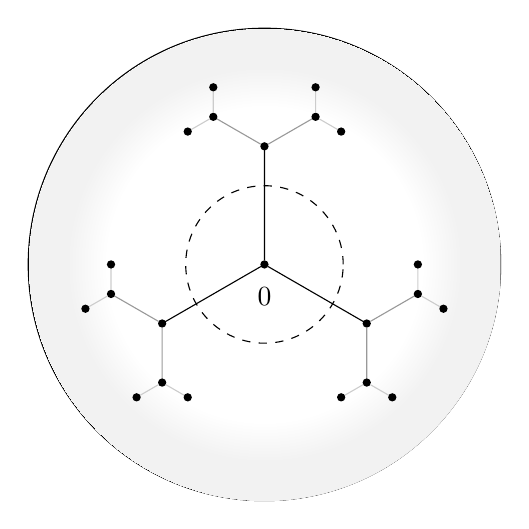
\begin{tikzpicture}[baseline=(current bounding box.center)]
% thanks to Tomasz M. Trzeciak
% based off of http://www.latex-community.org/viewtopic.php?f=4&t=2111

\draw (0,0) circle (3);

\begin{scope}
\pgfsetfading{fading3}{\pgftransformshift{\pgfpoint{0cm}{0cm}}}
\filldraw[black!5] (0,0) circle (3);
\end{scope}

\draw[dashed] (0,0) circle (1);
\coordinate[style={inner sep=0pt, outer sep=0pt, minimum size=3pt, fill=black, circle}] (O) at (0,0);
\node[below=5pt] at (O) {$0$};

\draw (O) -- +( 90:1.5) coordinate[style={inner sep=0pt, outer sep=0pt, minimum size=3pt, fill=black, circle}] (Q1)
      (O) -- +(210:1.5) coordinate[style={inner sep=0pt,outer sep=0pt,minimum size=3pt, fill=black,circle}] (Q2)
      (O) -- +(330:1.5) coordinate[style={inner sep=0pt,outer sep=0pt,minimum size=3pt, fill=black,circle}] (Q3);

\draw[black!40] (Q1) -- +(120-90:0.75) coordinate[style={inner sep=0pt, outer sep=0pt, minimum size=3pt, fill=black, circle}] (Q12)
      (Q1) -- +(240-90:0.75) coordinate[style={inner sep=0pt, outer sep=0pt, minimum size=3pt, fill=black, circle}] (Q13)
      (Q2) -- +(120-330:0.75) coordinate[style={inner sep=0pt, outer sep=0pt, minimum size=3pt, fill=black, circle}] (Q21)
      (Q2) -- +(240-330:0.75) coordinate[style={inner sep=0pt, outer sep=0pt, minimum size=3pt, fill=black, circle}] (Q23)
      (Q3) -- +(120-210:0.75) coordinate[style={inner sep=0pt, outer sep=0pt, minimum size=3pt, fill=black, circle}] (Q31)
      (Q3) -- +(240-210:0.75) coordinate[style={inner sep=0pt, outer sep=0pt, minimum size=3pt, fill=black, circle}] (Q32);

\draw[black!20] (Q12) -- +(90:0.375) coordinate[style={inner sep=0pt, outer sep=0pt, minimum size=3pt, fill=black, circle}] (Q121)
      (Q12) -- +(330:0.375) coordinate[style={inner sep=0pt, outer sep=0pt, minimum size=3pt, fill=black, circle}] (Q123)
      (Q13) -- +(90:0.375) coordinate[style={inner sep=0pt, outer sep=0pt, minimum size=3pt, fill=black, circle}] (Q131)
      (Q13) -- +(210:0.375) coordinate[style={inner sep=0pt, outer sep=0pt, minimum size=3pt, fill=black, circle}] (Q132)
      (Q21) -- +(90:0.375) coordinate[style={inner sep=0pt, outer sep=0pt, minimum size=3pt, fill=black, circle}] (Q212)
      (Q21) -- +(210:0.375) coordinate[style={inner sep=0pt, outer sep=0pt, minimum size=3pt, fill=black, circle}] (Q213)
      (Q23) -- +(210:0.375) coordinate[style={inner sep=0pt, outer sep=0pt, minimum size=3pt, fill=black, circle}] (Q231)
      (Q23) -- +(330:0.375) coordinate[style={inner sep=0pt, outer sep=0pt, minimum size=3pt, fill=black, circle}] (Q232)
      (Q31) -- +(210:0.375) coordinate[style={inner sep=0pt, outer sep=0pt, minimum size=3pt, fill=black, circle}] (Q312)
      (Q31) -- +(330:0.375) coordinate[style={inner sep=0pt, outer sep=0pt, minimum size=3pt, fill=black, circle}] (Q313)
      (Q32) -- +(90:0.375) coordinate[style={inner sep=0pt, outer sep=0pt, minimum size=3pt, fill=black, circle}] (Q321)
      (Q32) -- +(330:0.375) coordinate[style={inner sep=0pt, outer sep=0pt, minimum size=3pt, fill=black, circle}] (Q323);
\end{tikzpicture}%
%
\quad $\xrightarrow{\pi_{GH}}$ \quad%
%
\begin{tikzpicture}[baseline=(current bounding box.center)]

\newcommand\pgfmathsinandcos[3]{%
  \pgfmathsetmacro#1{sin(#3)}%
  \pgfmathsetmacro#2{cos(#3)}%
}
\newcommand\LongitudePlane[3][current plane]{%
  \pgfmathsinandcos\sinEl\cosEl{#2} % elevation
  \pgfmathsinandcos\sint\cost{#3} % azimuth
  \tikzset{#1/.style={cm={\cost,\sint*\sinEl,0,\cosEl,(0,0)}}}
}
\newcommand\DrawLongitudeCircle[2][1]{
  \LongitudePlane{35}{#2} % first argument is angle of elevation
  \tikzset{current plane/.prefix style={scale=#1}}
   % angle of "visibility"
  \pgfmathsetmacro\angVis{atan(sin(#2)*cos(35)/sin(35))} % these are angle of elevation too
  % this might assume that the angle of elevation is positive
  \draw[current plane] (\angVis:1) arc (\angVis:90:1);
  \draw[current plane,dashed] (\angVis:1) arc (\angVis:-90:1);
}

% the "2.5" magic number is the radius of the sphere 
% the "35" magic number is the angle of elevation of the camera
\pgfmathsetmacro\H{2.5*cos(35)}
\filldraw[ball color=white] (0,0) circle (2.5);
\foreach \t in {-5,-125,-245} { \DrawLongitudeCircle[2.5]{\t} }
\coordinate[style={inner sep=0pt,outer sep=0pt,minimum size=3pt,
    fill=black,circle}] (O) at (0,-\H);
\node[below=16pt] at (O) {$0$};
\coordinate[style={inner sep=0pt,outer sep=0pt,minimum size=3pt,
    fill=black,circle}] (I) at (0,\H);
\node[above=16pt] at (I) {$\infty$};
\end{tikzpicture}
\end{center}

\caption{The period map at $n = 2$, $p = 2$}
\end{figure}

\begin{theorem}\citeme{\cite{HopkinsGrossAnnouncement,StricklandGHDuality}}
\todo{Make sure you get this right.}
The sheaf $\context{E_\Gamma}(\mathbb I_{\Q/\Z})$ is the dualizing sheaf on $(\moduli{fg})^\wedge_\Gamma$. \qed
\end{theorem}





\section{Knowns and unknowns}



\subsection*{Higher orientations}

$\TAF$ and friends\label{TAFDiscussion}

The $\alpha_{1/1}$ argument: Prop 2.3.2 of Hovey's $v_n$--elements of ring spectra

% The HLP calculations

\subsection*{Equivariance}

This is tied up with the theory of power operations in a way I've never really thought about.  Seems complicated.

You should also mention the ``rigidity'' of the elliptic genus, which is about an $S^1$--equivariant version.

\subsection*{Index theorems}

Connections with analysis

The Stolz--Teichner program








-----

Bousfield's work on the $K$--theory of infinite loopspaces \cite{BousfieldLambdaRings} and Morava $K$--theoretic analogues of the results of \Cref{LEFTCooperations}
\todo{Ask Mike (and Jacob?) if there are analogues of these results for $kO$ which explain Mahowald's generalized $K$--theoretic Brown--Gitler spectra.  3/29: I did ask Mike, he said he didn't know. I also asked Paul, and he said this seemed unreasonable, since $kO$ isn't valued in co/commutative Hopf algebras.  This is a fair point: one would need to invent an ``analogue'' of Dieudonn\'e theory for $kO$, in the sense that some category it takes values in would have to be identified as abelian, where the category is rigid enough that it often sends fiber sequences to exact sequences in the category.}

Constructing sheaves of spectra on $\moduli{fg}$: the no-go results for $E_\infty$ and $A_\infty$ rings on the flat site.  There's a little MO discussion about it here: \texttt{http://chat.stackexchange.com/transcript/message/35361282\#35361282}.

Contexts for structured ring spectra

Difficulty in computing $\S_d \actson E_d^*$. (Gross--Hopkins and the period map.)

Barry's $p$--adic measures

Fixed point spectra and e.g. $L_{K(2)} \tmf$.

Blueshift, A--M--S, and the relationship to A--F--G?

Does $E_n$ receive an $E_\infty$ orientation?  Does $BP$?  (Johnson--Noel says $BP$ usually does not.  A recent preprint of Lawson says $BP$ is not even $E_\infty$ at $p = 2$!!!)

$p$--divisible groups and transchromatic phenomena

Remark 12.13 of published $H_\infty$ AHS says their obstruction framework agrees with the $E_\infty$ obstruction framework (if you take everything in sight to have $E_\infty$ structures).  This is almost certainly related to the discussion at the end of Matt's thesis about the $MU$--orientation of $E_d$.\todo{Section 12.4 compares doing $H_\infty$ descent with doing $E_\infty$ descent and shows that they're the same (in the case of interest?).}

Hovey's paper on $v_n$--periodic elements in ring spectra.  He has a nice (and thorough!) exposition on why one should be interested in bordism spectra and their splittings: for instance, a careful analysis of $M\Spin$ will inexorably lead one toward studying $KO$.  It would be nice if studying $M\String$ (and potentially higher analogues) would lead one toward non-completed, non-connective versions of $EO_n$.  Talk about $BoP$, for instance.

Matt's short resolutions of chromatically localized $MU$.

Nilpotency and vanishing curves in the ($MU$--)Adams spectral sequence.  The \emph{non}-nilpotency of $\eta$ in the $MU$--Adams spectral sequence.  Mathew--Meier type theorems about horizontal vanishing lines and the Tate construction (and related results about the $\TMF$ spectral sequence and the Johnson--Wilson theories).

Additive degeneration and $kO \ne kU^{hC_2}$.






\begin{remark}
It is completely unclear why $MU$ plays such an important mediating role between geometry (i.e., the stable category) and algebra (i.e., sheaves on the moduli of formal groups).  Given a general ring spectrum $R$ and thick prime $\otimes$--ideals $\CatOf C_\alpha$ of perfect $R$--modules, one ask the analogous two questions:
\begin{enumerate}
\item Is it possible to find an $R$--algebra $S$ whose context functor induces a homeomorphism of Balmer spectra $\Spec(\CatOf{Modules}_R^{\perf}) \to \Spec(\CatOf{QCoh}(\context{S/R}))$?
\item Are there complementary localizers $L_\alpha\co \CatOf{Modules}_R \to \CatOf{Modules}_{R,(\alpha)}$?  Can they be presented via Bousfield's framework as homological localizations for auxiliary $S$--algebra spectra $S_\alpha$?  Do the contexts $\context{S_\alpha}$ admit compatible localizers with $\context{S}$?
\end{enumerate}
For $R = \S$, this is the role that the $R$--algebra $S = MU$ and the $S$--algebras $S_d = E(d)$ play.  Finding these spectra feels like striking gold, and it is unclear how to produce analogous spectra in general.
\todo{Mathews's work on Galois descent shows that the fixed point map $\CatOf{Modules}_{E_\Gamma, \Aut \Gamma}^{\mathrm{complete}} \to \CatOf{Spectra}_{\Gamma}$ is an equivalence of categories.}
\end{remark}
\noindent One can ask the same question from the geometric direction: why bordism?  Why should these spectra have these nice flatness properties?  Why should they have recognizable computational properties?  Why bordism?




\begin{remark}
The homotopy of $\widehat L_2 \S$ is also known, by work of Shimomura and collaborators~\cite{Shimomura,ShimomuraYabeM20,ShimomuraYabeL2S} (but see also the reorganization by Behrens~\cite{BehrensRevisited}).  It is \emph{exceedingly} complicated, and it is an open problem to find an expression of it which admits human digestion.  Behrens has pursued a program encoding this problem in terms of modular forms~\cite{BehrensCongruences,BehrensModularDescription,BehrensBuildings}, and Hopkins has proposed a program involving $L$--functions~\cite{StricklandpAdicInterpolation}, motivated by which Hovey and Strickland have shown a kind of continuity result for among the groups~\cite[Section 14]{HoveyStrickland}.
\end{remark}





\begin{remark}
There are also ``finitary'' flavors of chromatic localization available, which are typically less robust but more computable.  They assemble into a diagram:
\begin{center}
\begin{tikzcd}
E \arrow{r} \arrow{d} & L_d^{\fin} E \arrow{r} \arrow{d} & L_d E \arrow{d} \\
L_{X(d)} E \arrow{r} & \widehat L_d^{\fin} E \arrow{r} & \widehat L_d E,
\end{tikzcd}
\end{center}
where $X(d)$ is a finite complex of type exactly $d$, $v$ is a $v_d$--self-map of $X(d)$, $T(d) = X(d)[v^{-1}]$ is the localizing telescope, $\widehat L_d^{\fin}$ is Bousfield localization with respect to $T(d)$ (which can be shown to be independent of choice of $X(d)$ and of $v$), and $L_d^{\fin}$ denotes localization with respect to the class of \emph{finite} $E(d)$--acyclics.  Many things about these functors are known: for instance, $L_{X(d)} L_d = \widehat L_d$, there is a chromatic fracture square relating $L_d^{\fin}$ to $\widehat L_{\le d}^{\fin}$, and $L_d^{\fin} E \simeq L_d E$ if and only if $\widehat L_{\le d}^{\fin} E \simeq \widehat L_{\le d} E$.  One major question about these functors remains open, corresponding the last unsettled nilpotence and periodicity conjecture of Ravenel~\cite[Conjecture 10.5]{RavenelLocalizationWRTPeriodic}: is the map $\widehat L_d^{\fin} E \to \widehat L_d E$ an equivalence?  Multiple proofs and disproofs have been offered, but the literature remains unsettled.
\citeme{Find some proofs and disproofs.}
\end{remark}







\begin{remark}
Writing $M_d$ for the fiber in the sequence $M_d \to L_d \to L_{d-1}$, the filtration spectral sequence associated to the tower in \Cref{ChromaticConvergence} is called the \textit{geometric chromatic spectral sequence}, which has the form $\pi_* M_* \S \Rightarrow \pi_* \S_{(p)}$.  The two forms of filtration data $M_d X$ and $\widehat L_d X$ are actually functorially equivalent to one another:
\begin{align*}
\widehat L_d M_d & \simeq \widehat L_d, &
M_d \widehat L_d & \simeq M_d,
\end{align*}
but they have fairly distinct properties.  For instance, $M_d$ is smashing whereas $\widehat L_d$ is not, $M_d$ is not part of an adjoint pair whereas $\widehat L_d$ is, and the analogue of \Cref{FormulaForKnLocalization} for $M_d$ is ``backwards'':\citeme{I forget who this is due to} \[M_d X \simeq \colim_I \left( M^0(v^I) \sm L_d X \right).\]  The spectrum $M_d X$ also relates to the chromatic fracture square for $X$:
\begin{center}
\begin{tikzcd}
M_d X \arrow{d} \arrow[equal]{r} & M_d X \arrow{d} \\
L_d X \arrow{r} \arrow{d} \arrow[dr, phantom, "\lrcorner", very near start] & \widehat L_d X \arrow{d} \\
L_{d-1} X \arrow{r} & L_{d-1} \widehat L_d X.
\end{tikzcd}
\end{center}
From this, we see that there is a fiber sequence $M_d X \to \widehat L_d X \to L_{d-1} \widehat L_d X$.

The case $d = 1$ gives the prototypical example of the difference between these two presentations of the ``exact height $d$ data'', where the sequence becomes: \[\colim_j (M^0(p^j) \sm L_1 X) \to \lim_j (M_0(p^j) \sm L_1 X) \to \left( \lim_j (M_0(p^j) \sm L_1 X) \right)_{\Q}.\]  If, for instance, $\pi_0 L_1 X = \Z_{(p)}$, then the long exact sequence of homotopy groups associated to this fiber sequence gives
\begin{center}
\begin{tikzcd}
\pi_0 \widehat L_1 X \arrow{r} \arrow[equal]{d} & \pi_0 L_0 \widehat L_1 X \arrow{r} \arrow[equal]{d} & \pi_{-1} M_1 X \arrow[equal]{d} \\
\Z^\wedge_p \arrow{r} & \Q_p \arrow{r} & \Z/p^\infty.
\end{tikzcd}
\end{center}
Coupling this to \Cref{piLK1SExample}, we compute
\begin{align*}
\pi_t M_1 \S^0 & = \begin{cases} \Z/p^\infty & \text{when $t = -1$}, \\ \Z_p / (pk) & \text{when $t = k|v_1| - 1$ and $t = \ne 0$}, \\ \Z/p^\infty & \text{when $t = (0 \cdot |v_1| - 1) - 1 = -2$}, \\ 0 & \text{otherwise}. \end{cases}
\end{align*}
This is a model for what happens generally when passing from $\pi_* \widehat L_d X$ to $\pi_* M_d X$: the $v_j$--torsion--free groups get converted to infinitely $v_j$--divisible groups, with some dimension shifts.\footnote{A height $2$ example of this same phenomenon is visible in Behrens's paper~\cite[Section 7]{BehrensRevisited}.}
\end{remark}




\begin{theorem}[Unpublished work of Hopkins and Lurie]
Let $F_d$ denote the discrepancy spectrum for $E_d$.  There is a natural equivalence of infinite loopspaces $\Loops^\infty F_d \simeq \Susp^d \mathbb I_{\Q/\Z}$. \qed
\end{theorem}




free $E_\infty$--orientations off of $MU$



At the top fo page 10 Neil talks in FPFP very briefly about Greenlees--May and local homology.






Comparison of comodules $M$ for the isogenies pile with the action of $M_n(\Z_p)$ on $M \otimes_{E_n^*} D_\infty$ (this is a modern result due to Tomer, Tobi, Lukas, and Nat).  This is basically Nat's rational claim: start with a sheaf on the isogenies pile.  Tensor everything with $\Q$.  That turns this thing into a rational algebra under the Drinfel'd ring together with an equivariant action of $\GL_n \Q_p$.





\todo[inline]{Leave a remark in here about this: McClure in BMMS works along similar lines to show that the Quillen idempotent is not $H_\infty$, but he doesn't get any positive results (and, in particular, he can't complete his analysis as we do because he doesn't have access to the $BP$--homology of finite groups and to HKR character theory).  One wonders whether the stuff here does say something about $BP$ as the height tends toward $\infty$.  So far as I know, no one has written much about this.  Surely it remains a bee in Matt's bonnet.}







Sections 5.3-4 of Hopkins's ICM address \textit{Algebraic Topology and Modular Forms} has a discussion of what $\eta$ and $\nu$ have to do with $\tmf$, as well as the construction of some interesting ``topological $\theta$--series'' in the elliptic cohomology of certain Thom complexes.



\todo[inline]{Jacob wrote me an email giving a very slightly fuller sketch of what the DAG perspective on the $\sigma$--orientation is.  Interestingly, it boils down to a fact from projective geometry: there just aren't that many line bundles on projective varieties.  This forces a couple of things to become equal, and in a suitable setting they even become canonically equal.  The email has no subject line, which will make it hard to find, but you should include a summary of it (which is dependent on whatever's written in the \textit{Survey} paper) all the same.}



